\documentclass[review]{elsarticle}

\usepackage{lineno,hyperref}

\usepackage{graphicx}% Include figure files
\usepackage{dcolumn}% Align table columns on decimal point
\usepackage{amsmath}
\usepackage{amssymb}
\usepackage{epstopdf}
\usepackage{multirow}
\usepackage{color}
\usepackage{longtable}
\usepackage{braket}
%\usepackage{hepparticles} % particle names
%\usepackage{hepnames} % shortcuts for lots of particle names
\usepackage[alsoload=hep]{siunitx}

\sisetup{ per-mode=symbol}


\graphicspath{{figures/}}

\modulolinenumbers[5]

\journal{}
\bibliographystyle{elsarticle-num}


%%%%%%%%%%%%%%%%%%%%%%%%%%%%%%%%%%%%%%%%%%%% 
\newcommand*{\MIT }{Massachusetts Institute of Technology, Cambridge, Massachusetts 02139, USA}
\newcommand*{\ODU}{Old Dominion University, Norfolk, Virginia 23529}
\newcommand*{\JLAB}{Thomas Jefferson National Accelerator Facility, Newport News, Virginia 23606}
\newcommand*{\TAU }{School of Physics and Astronomy, Tel Aviv University, Tel Aviv 69978, Israel}
\newcommand*{\Penn}{Pennsylvania State University, University Park, PA, 16802}


\begin{document}


%%%%%%%%%%%%%%%%%%%%%%%%%%%%%%%%%%%%%%%%%%%%%%%%%%%%%%%%%%%%%%%%%%%%%%%%%%%%%%%%%%%%%%%%%%%%%%%%%%%
\begin{frontmatter}

\title{The CLAS12 Backward Angle Neutron Detector (BAND) for high momentum neutrons}

%% Group authors per affiliation:
\author{E.P.~Segarra, F.~Hauenstein, A.~Schmidt, R.~Cruz-Torres, \\O.~Hen, A.~Denniston, T.~Kutz, J.~Pybus, A.~Hrnjic\\A.~Nambrath\corref{mycorrespondingauthor}}
\address{\MIT}
\author{C.~Fogler, L.B.~Weinstein, T.~Hartlove}
\address{\ODU}
\author{E.~Piasetzky}
\address{\TAU}
\author{K.~Pryce}
\address{Orsay}
\author{P.~Eugenio}
\address{FSU}
\author{I.~Vega, M.~Mu\~nos, H.~Hakobyan}
\address{UTFSM}
\author{A.~Beck, S.~Beck}
\address{}
\author{P.~Correa}
\address{}
\author{People from JLab?}
\address{}

%%%%%%%%%%%%%%%%%%%%%%%%%%%%%%%%%%%%%%%%%%%%%%%%%%%%%%%%%%%%%%%%%%%%%%%%%%%%%%%%%%%%%%%%%%%%%%%%%%%
\author[]{}
\ead[]{}

\begin{abstract}
The Backward Angle Neutron Detector (BAND) of CLAS12 is discussed. The detector is positioned $3$ \si{\meter} upstream of the target to 
detect backward neutrons with momenta between $0.25$ and $0.7$ \si{\GeV/\clight}. It consists of $18$ rows and $5$ layers of $7.2$ \si{\centi\meter} 
by $7.2$ \si{\centi\meter} scintillator bars with PMT readout on both ends to measure the neutron time-of-flight from the target and the 
energy deposition in the scintillator layers. There is an additional $1$ \si{\centi\meter} veto layer for vetoing charged particles. The detector 
covers an angular range of backward going particles from $155$\si{\degree} to $175$\si{\degree} with a detection efficiency of 
$35$\% and momentum resolution of $<1.5$\%.
\end{abstract}

\begin{keyword}
CLAS12; Time of flight; Plastic scintillator; Fast neutrons
\end{keyword}
\end{frontmatter}

%%%%%%%%%%%%%%%%%%%%%%%%%%%%%%%%%%%%%%%%%%%%%%%%%%%%%%%%%%%%%%%%%%%%%%%%%%%%%%%%%%%%%%%%%%%%%%%%%%%
\linenumbers

\section{Overview of CLAS12}


The CLAS12 (Cebaf Large Angle Spectrometer)[ADD REF] in Jefferson Lab's HallB experimental hall is a multi-purpose spectrometer to detect charged and neutral particles. It covers angles from xx to xx and momenta from xx to xx for the different particles. For our physics of interest, it is necessary to detect recoil neutrons with momenta above \SI{200/250}{\mega\eVperc} at backward angles. Therefore, a new detector has been build to detect these neutrons, the Backward Angle Neutron Detector (BAND); see Fig.~\ref{fig:clas12}.

\begin{figure}[h]
	\centering
	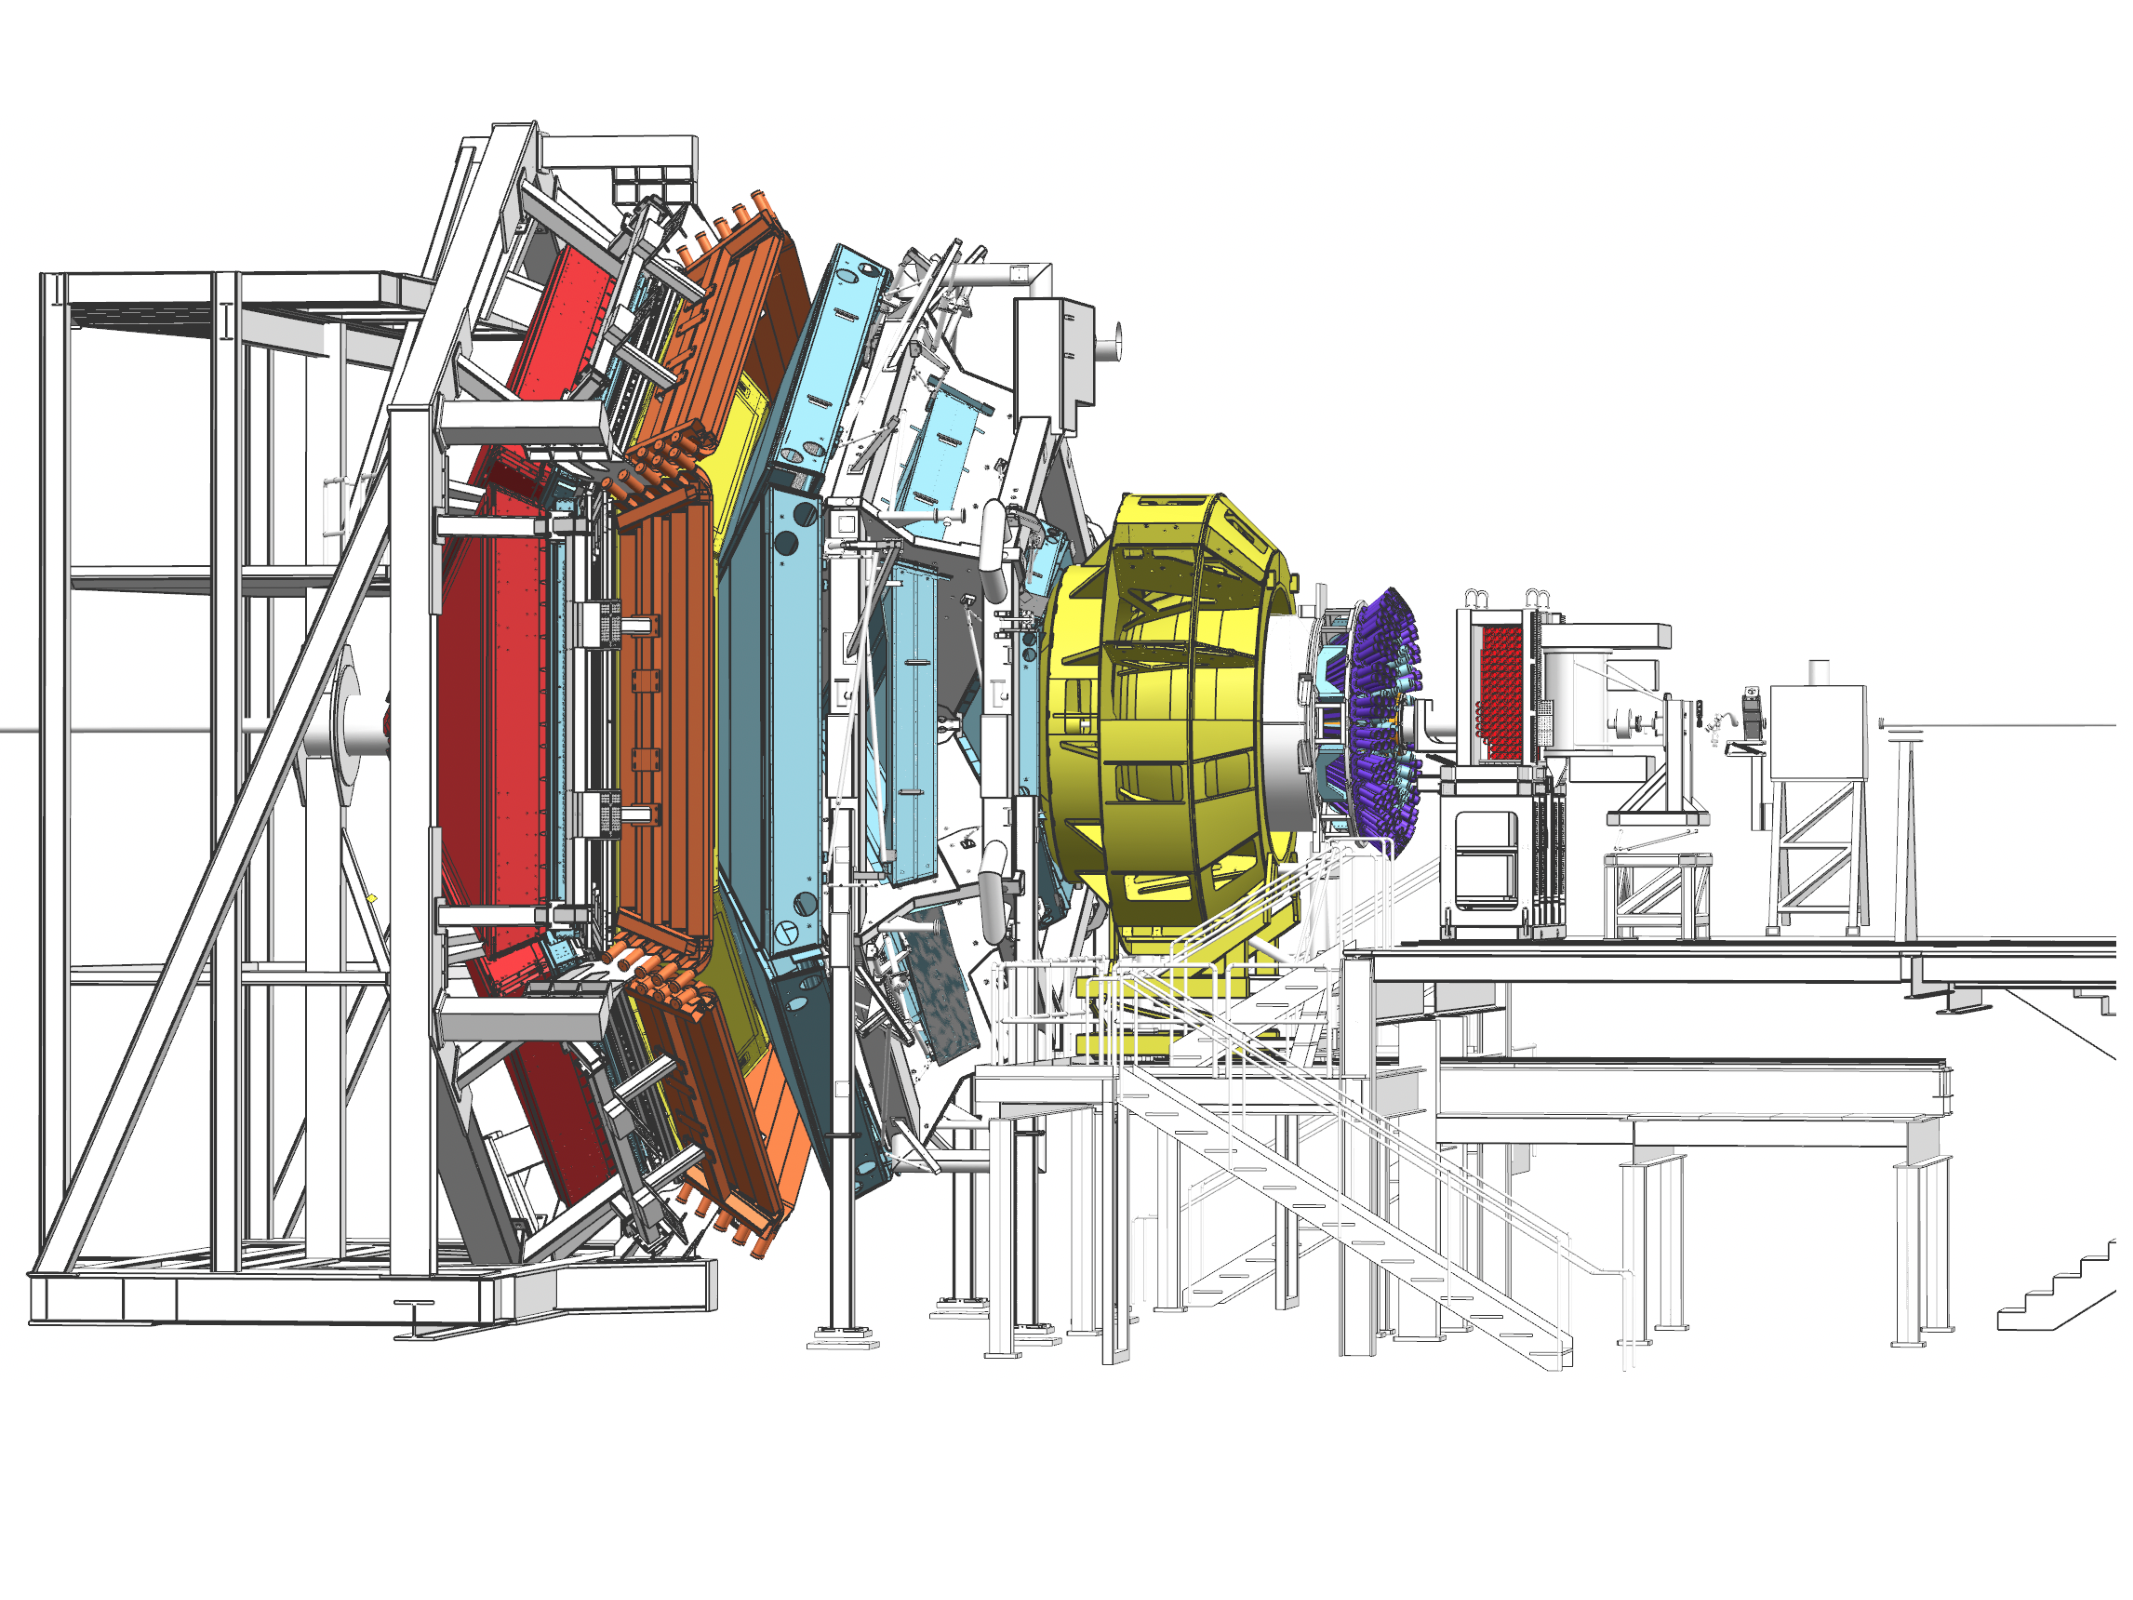
\includegraphics[width=0.48\textwidth]{BandInClas.pdf}
	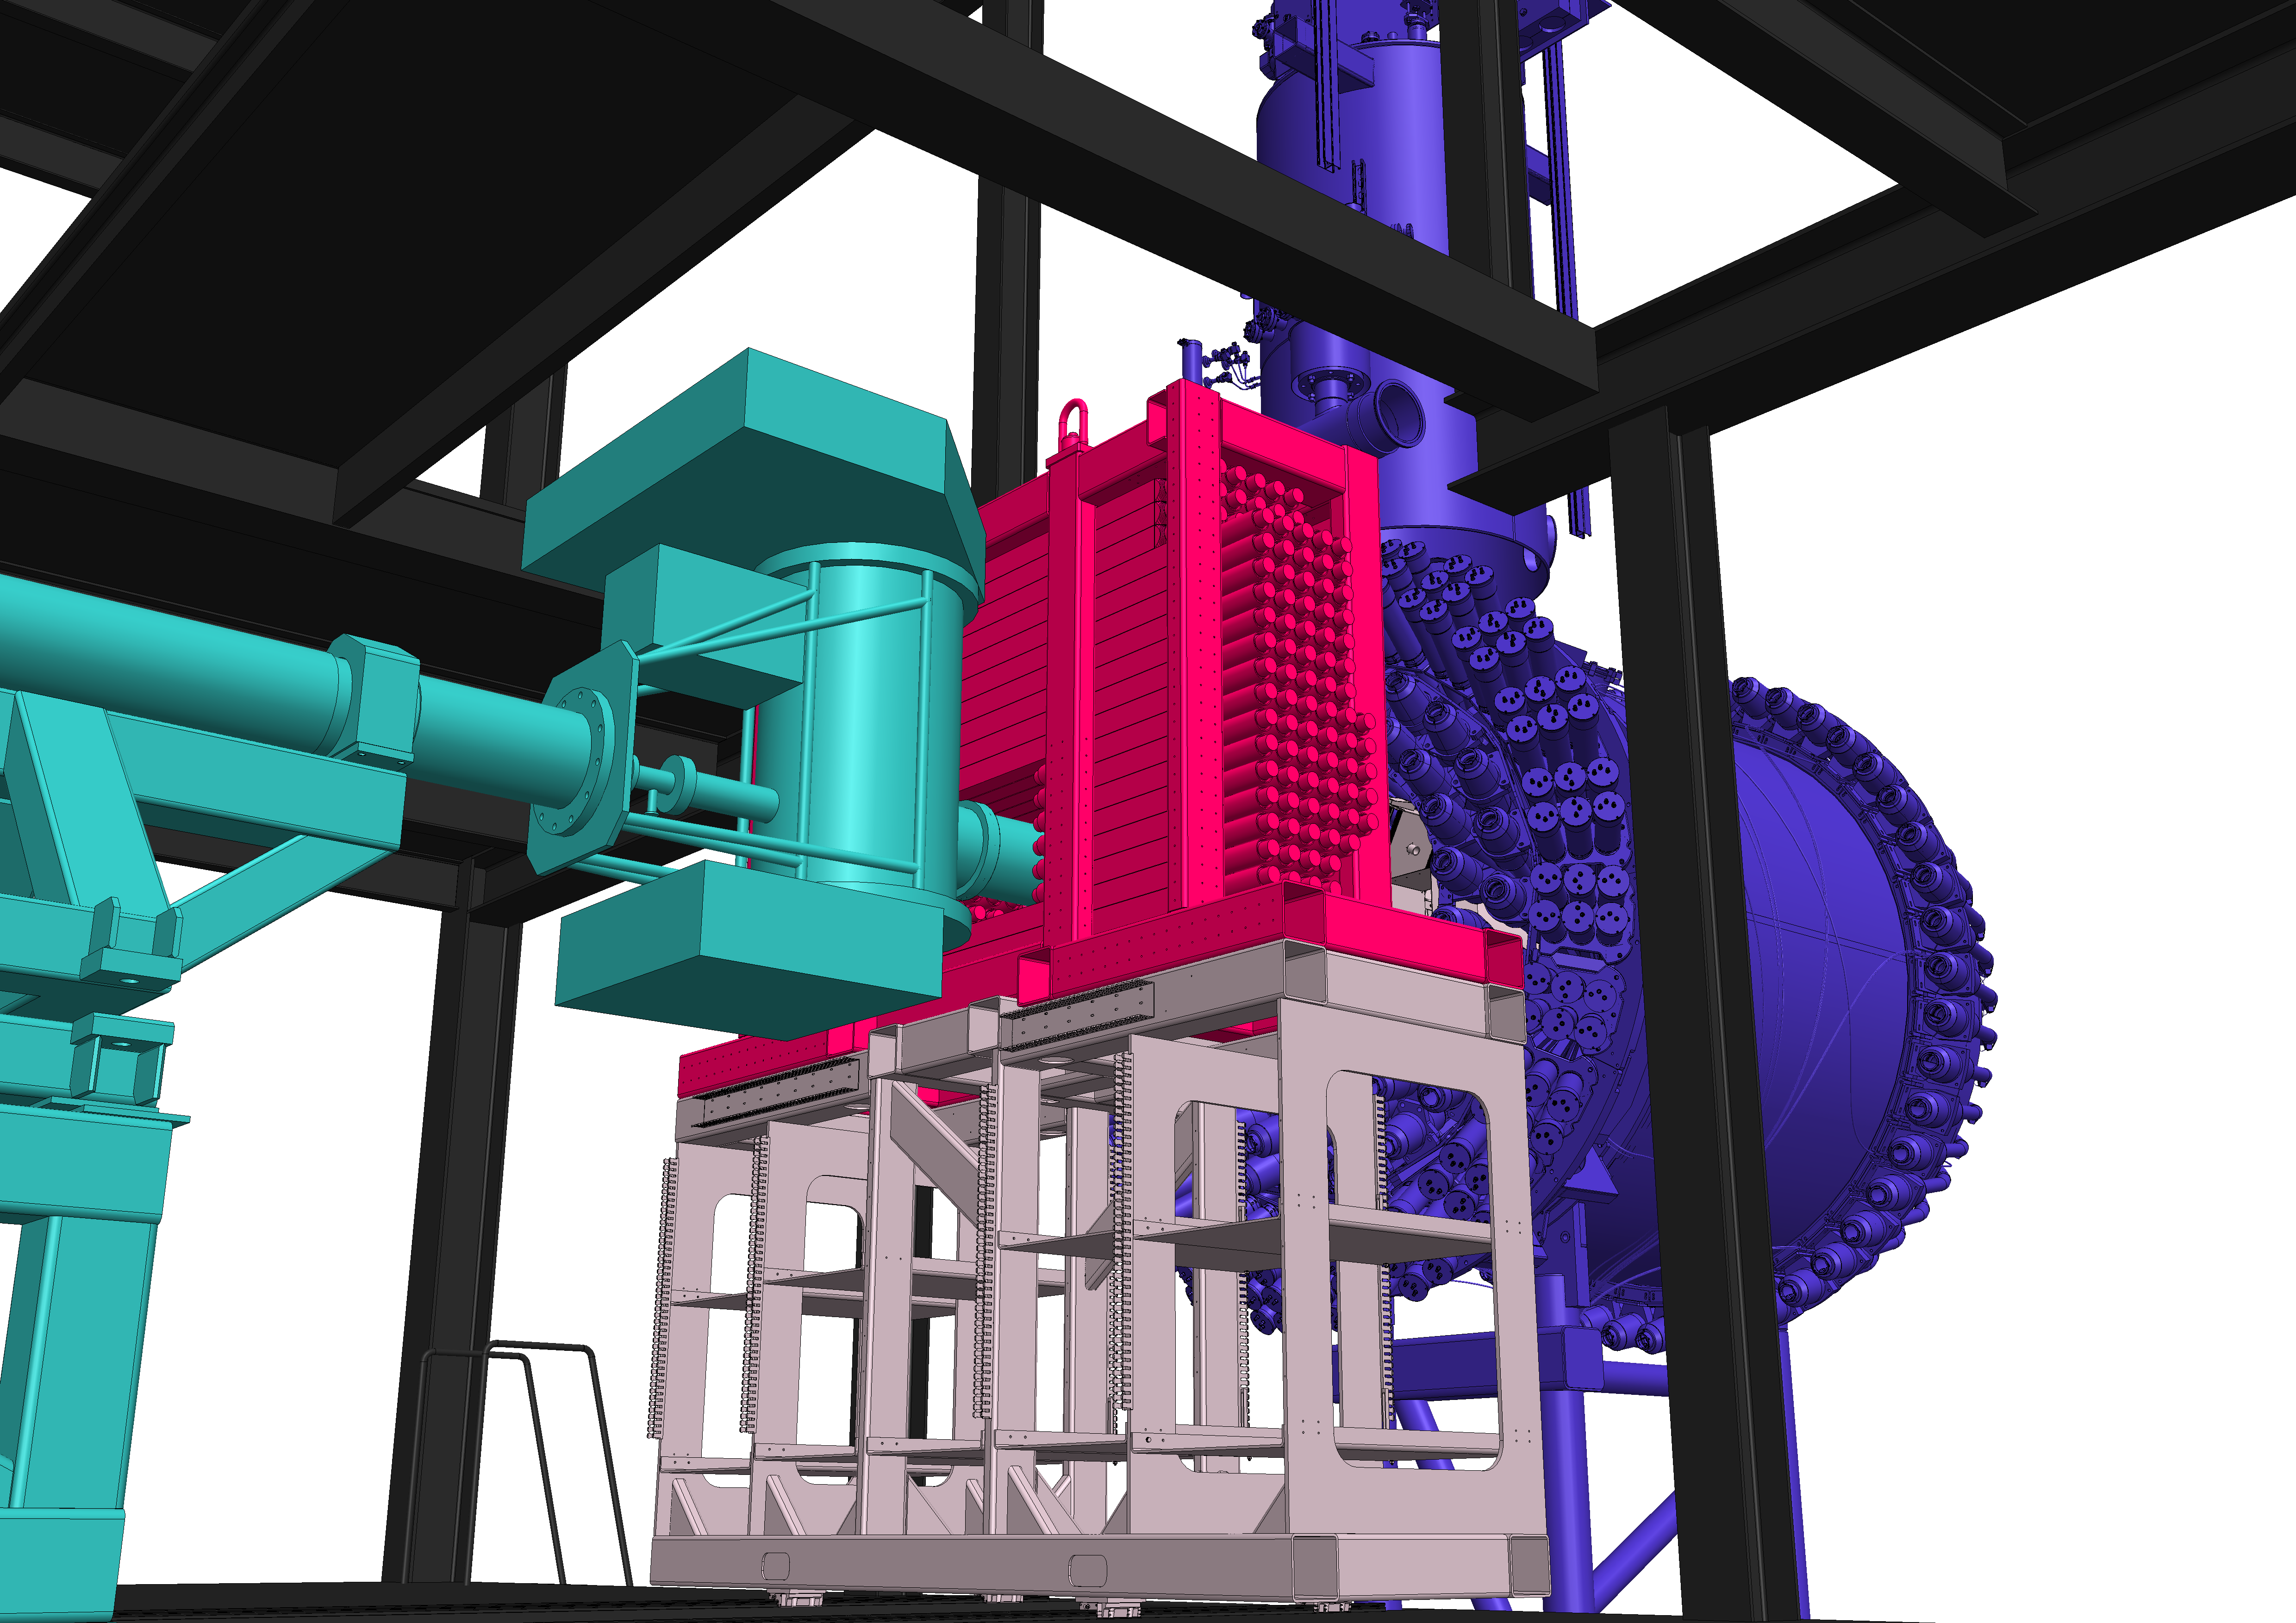
\includegraphics[width=0.48\textwidth]{FULL_CONTEXT_STUDIE_3.png}
	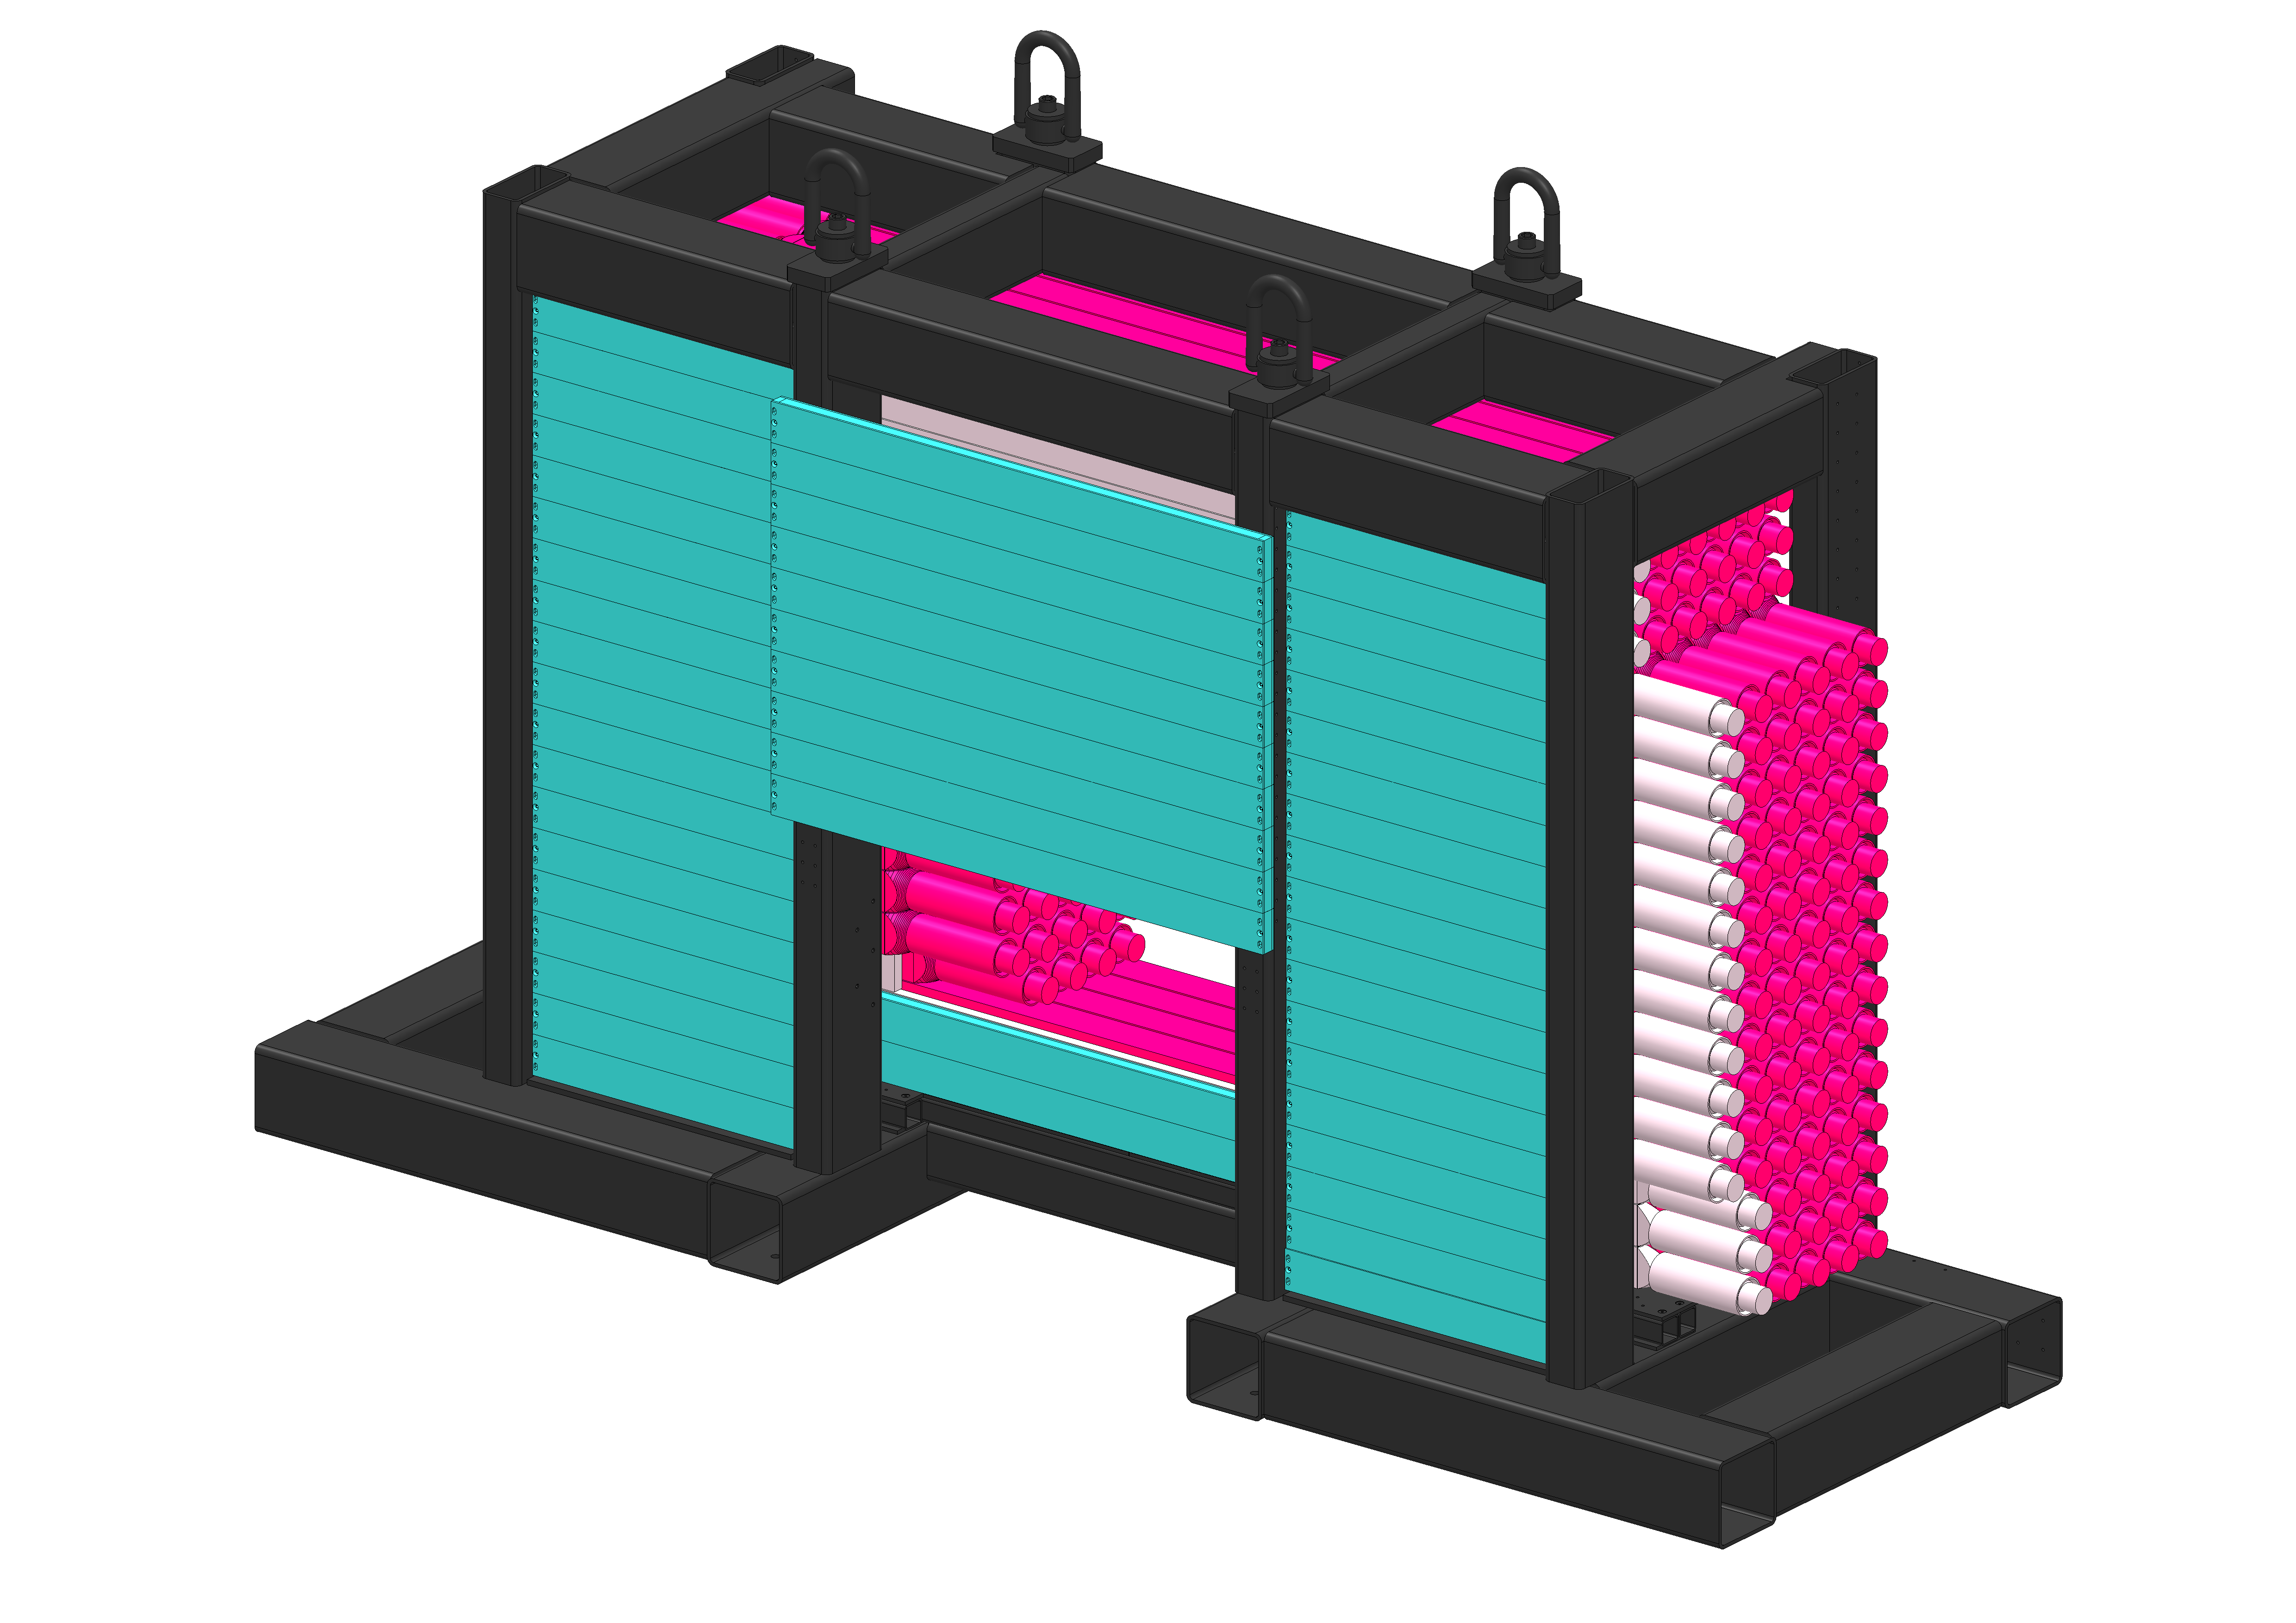
\includegraphics[width=0.48\textwidth]{BAND_1-2.png}
		\caption{BAND with CLAS12}
		\label{fig:clas12}
\end{figure}


%%%%%%%%%%%%%%%%%%%%%%%%%%%%%%%%%%%%%%%%%%%%%%%%%%%%%%%%%%%%%%%%%%%%%%%%%%%%%%%%%%%%%%%%%%%%%%%%%%%

\section{Design of the backward angle neutron detector}
To achieve the physics channels of interest with neutrons in the BAND, time-of-flight (ToF) resolutions below $300$ \si{\pico\second} and XXX path length 
resolution are required for the scintillant detector {\color{red}(and neutron PID?)}. {\color{red}These design parameters... (why are these the 
design parameters)}. Neutral-particle identification is established via vetoing algorithms ({\color{red}see online supplemental materials}) aided by
a thin $1$ \si{\centi\meter} veto layer for charged-particle identification. Neutron-photon discrimination is achieved with ToF separation given the design 
timing resolutions. Furthermore, off-time random neutron contamination can be controlled with signal energy deposit. {\color{red} Any need to mention 
the raw rates that we need to handle in CLAS12?} 

\subsection{Geometry}
The geometry of the BAND was constrained by the physics of interest (i.e. backward-going neutrons) \cite{Emcsrcdeens} and the available space in the hall. To
maximize the fiducial volume inside of hall constraints, a design of rectangular scintillant bars that are layered in $z$ and $y$ was chosen; see Fig.~\ref{fig:design}.
The cross section of each scintillator bar determines our position granularity in $y,z$, and was chosen such that it yields comparable uncertainty to $x$ given the bar 
time resolutions. With a design ToF resolution below $300$ \si{\pico\second}, $7.2$ \si{\centi\meter} by $7.2$ \si{\centi\meter} scintillator bars were chosen to optimize
fiducial volume, granularity, and cost.
\begin{figure}[h]
	\centering
		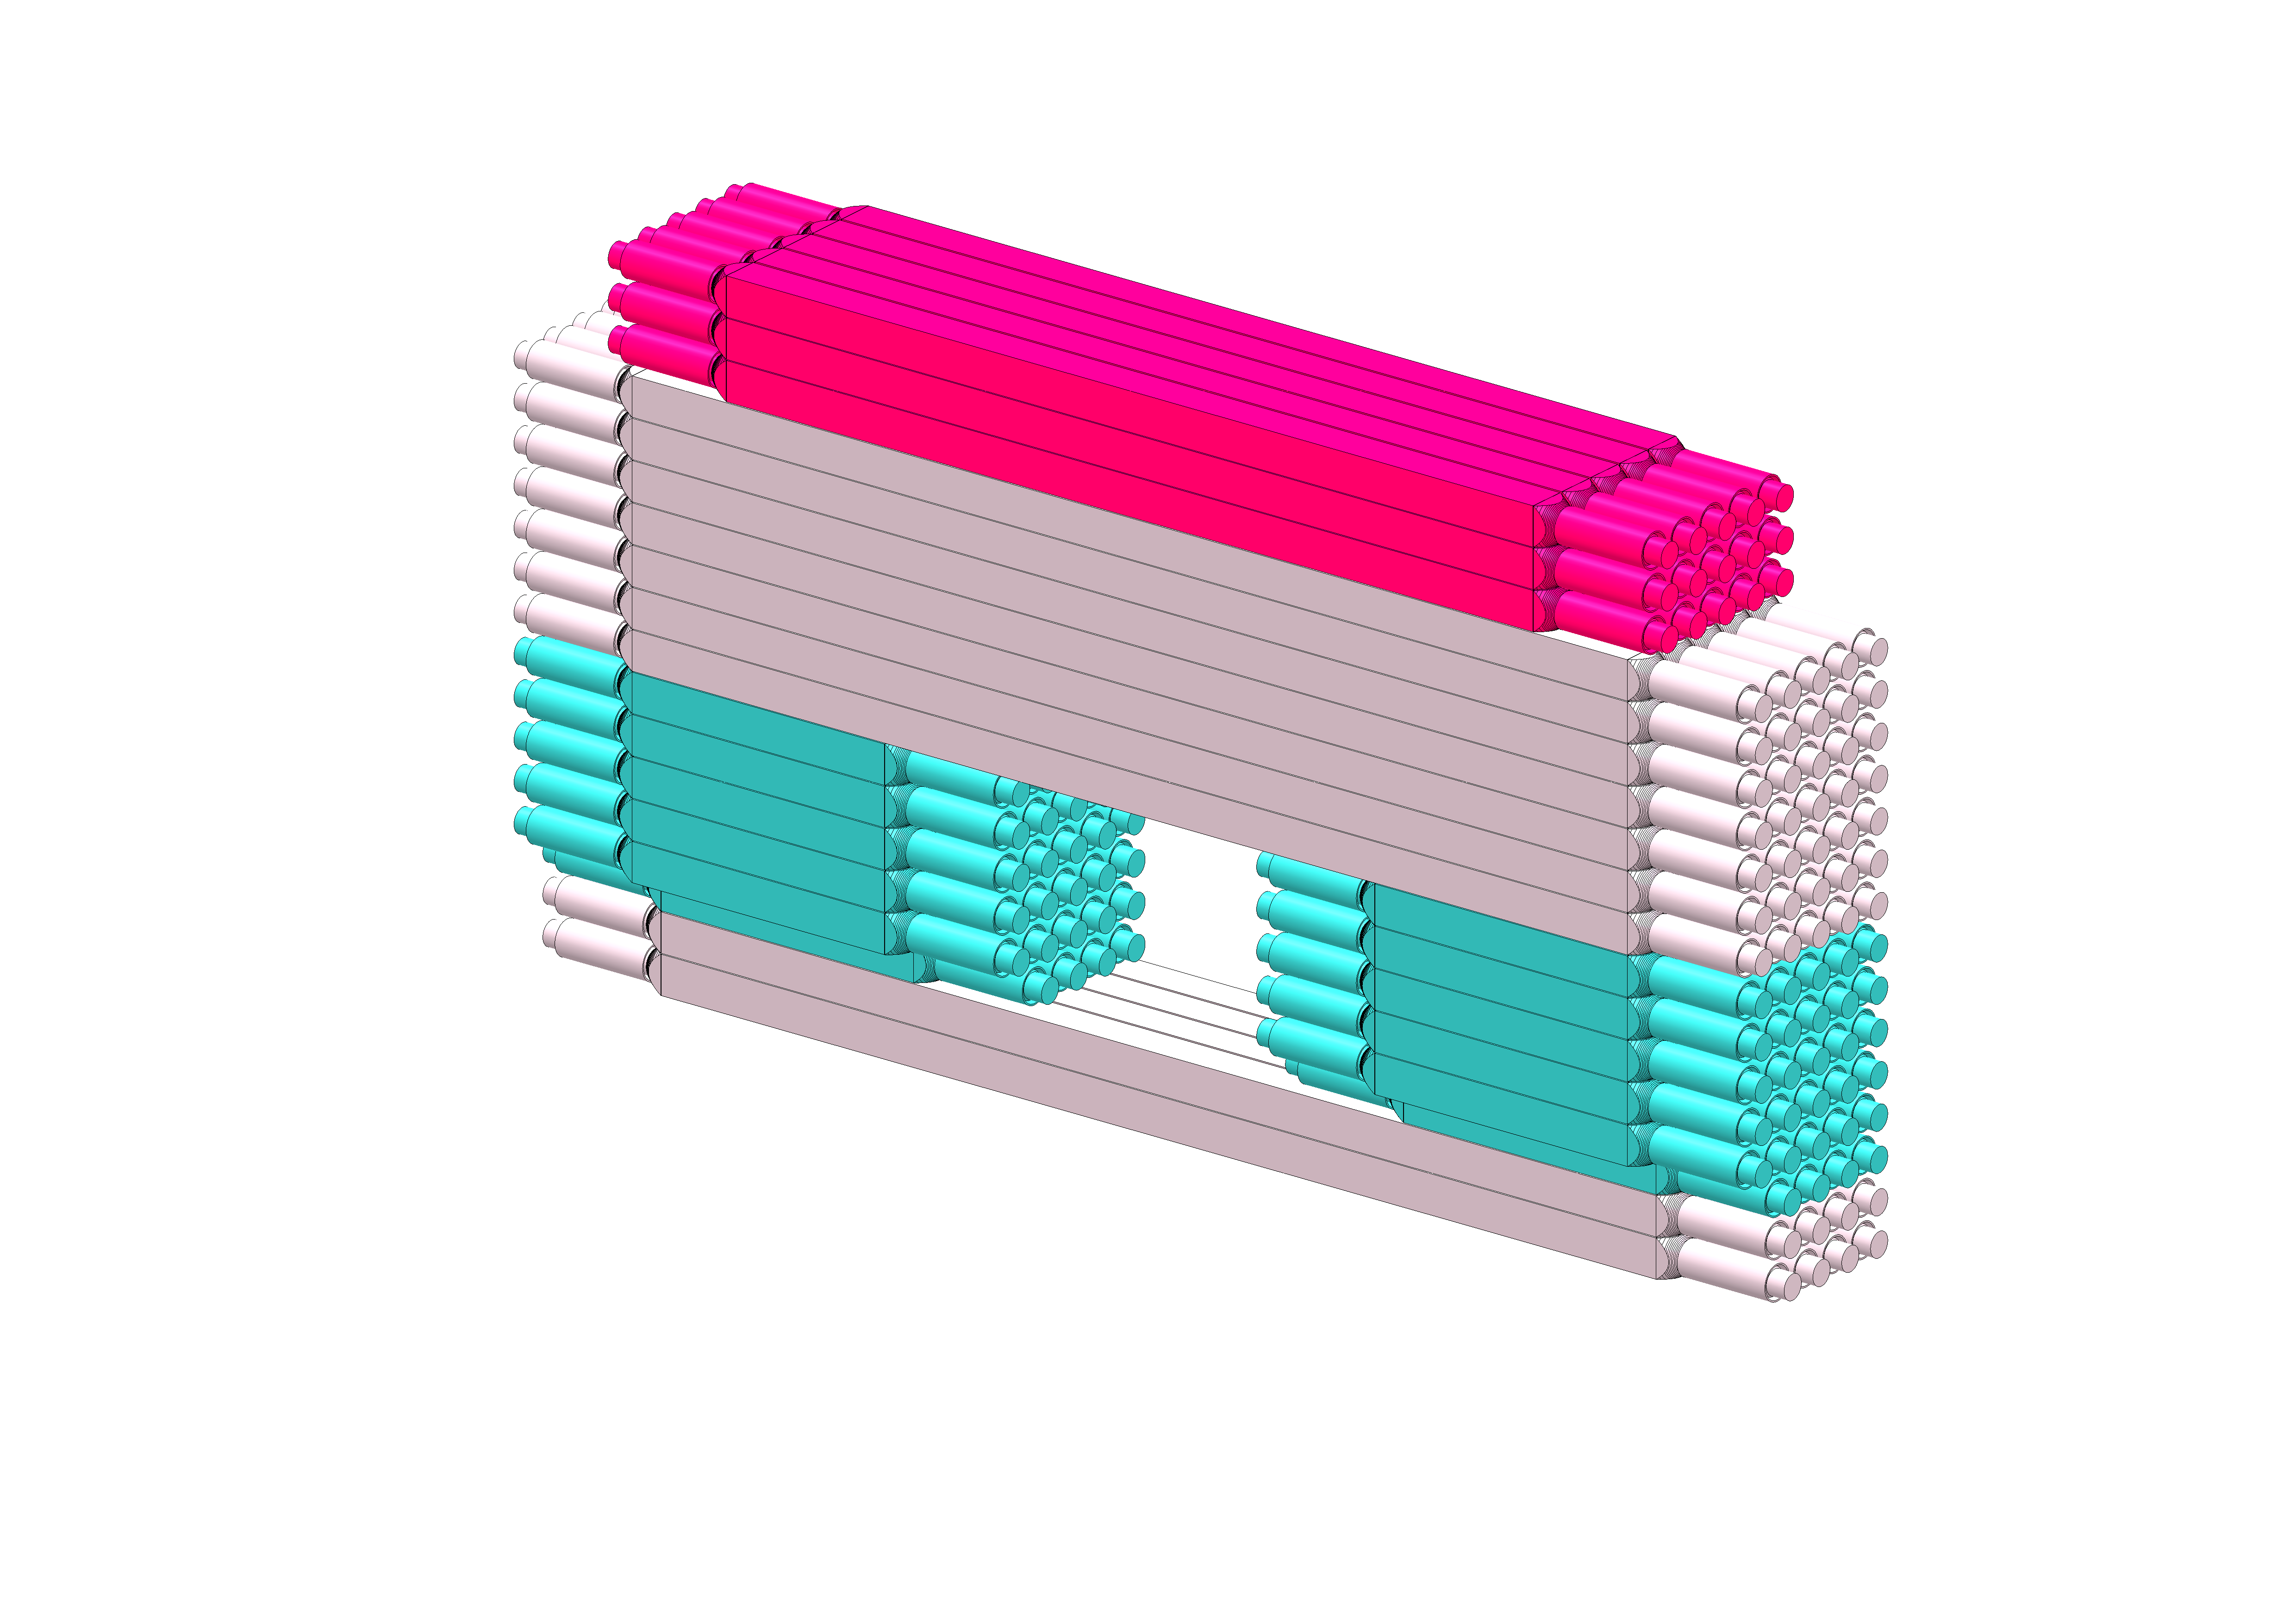
\includegraphics[width=0.48\textwidth]{MAIN_DETECTOR_COLORED_2.png}
		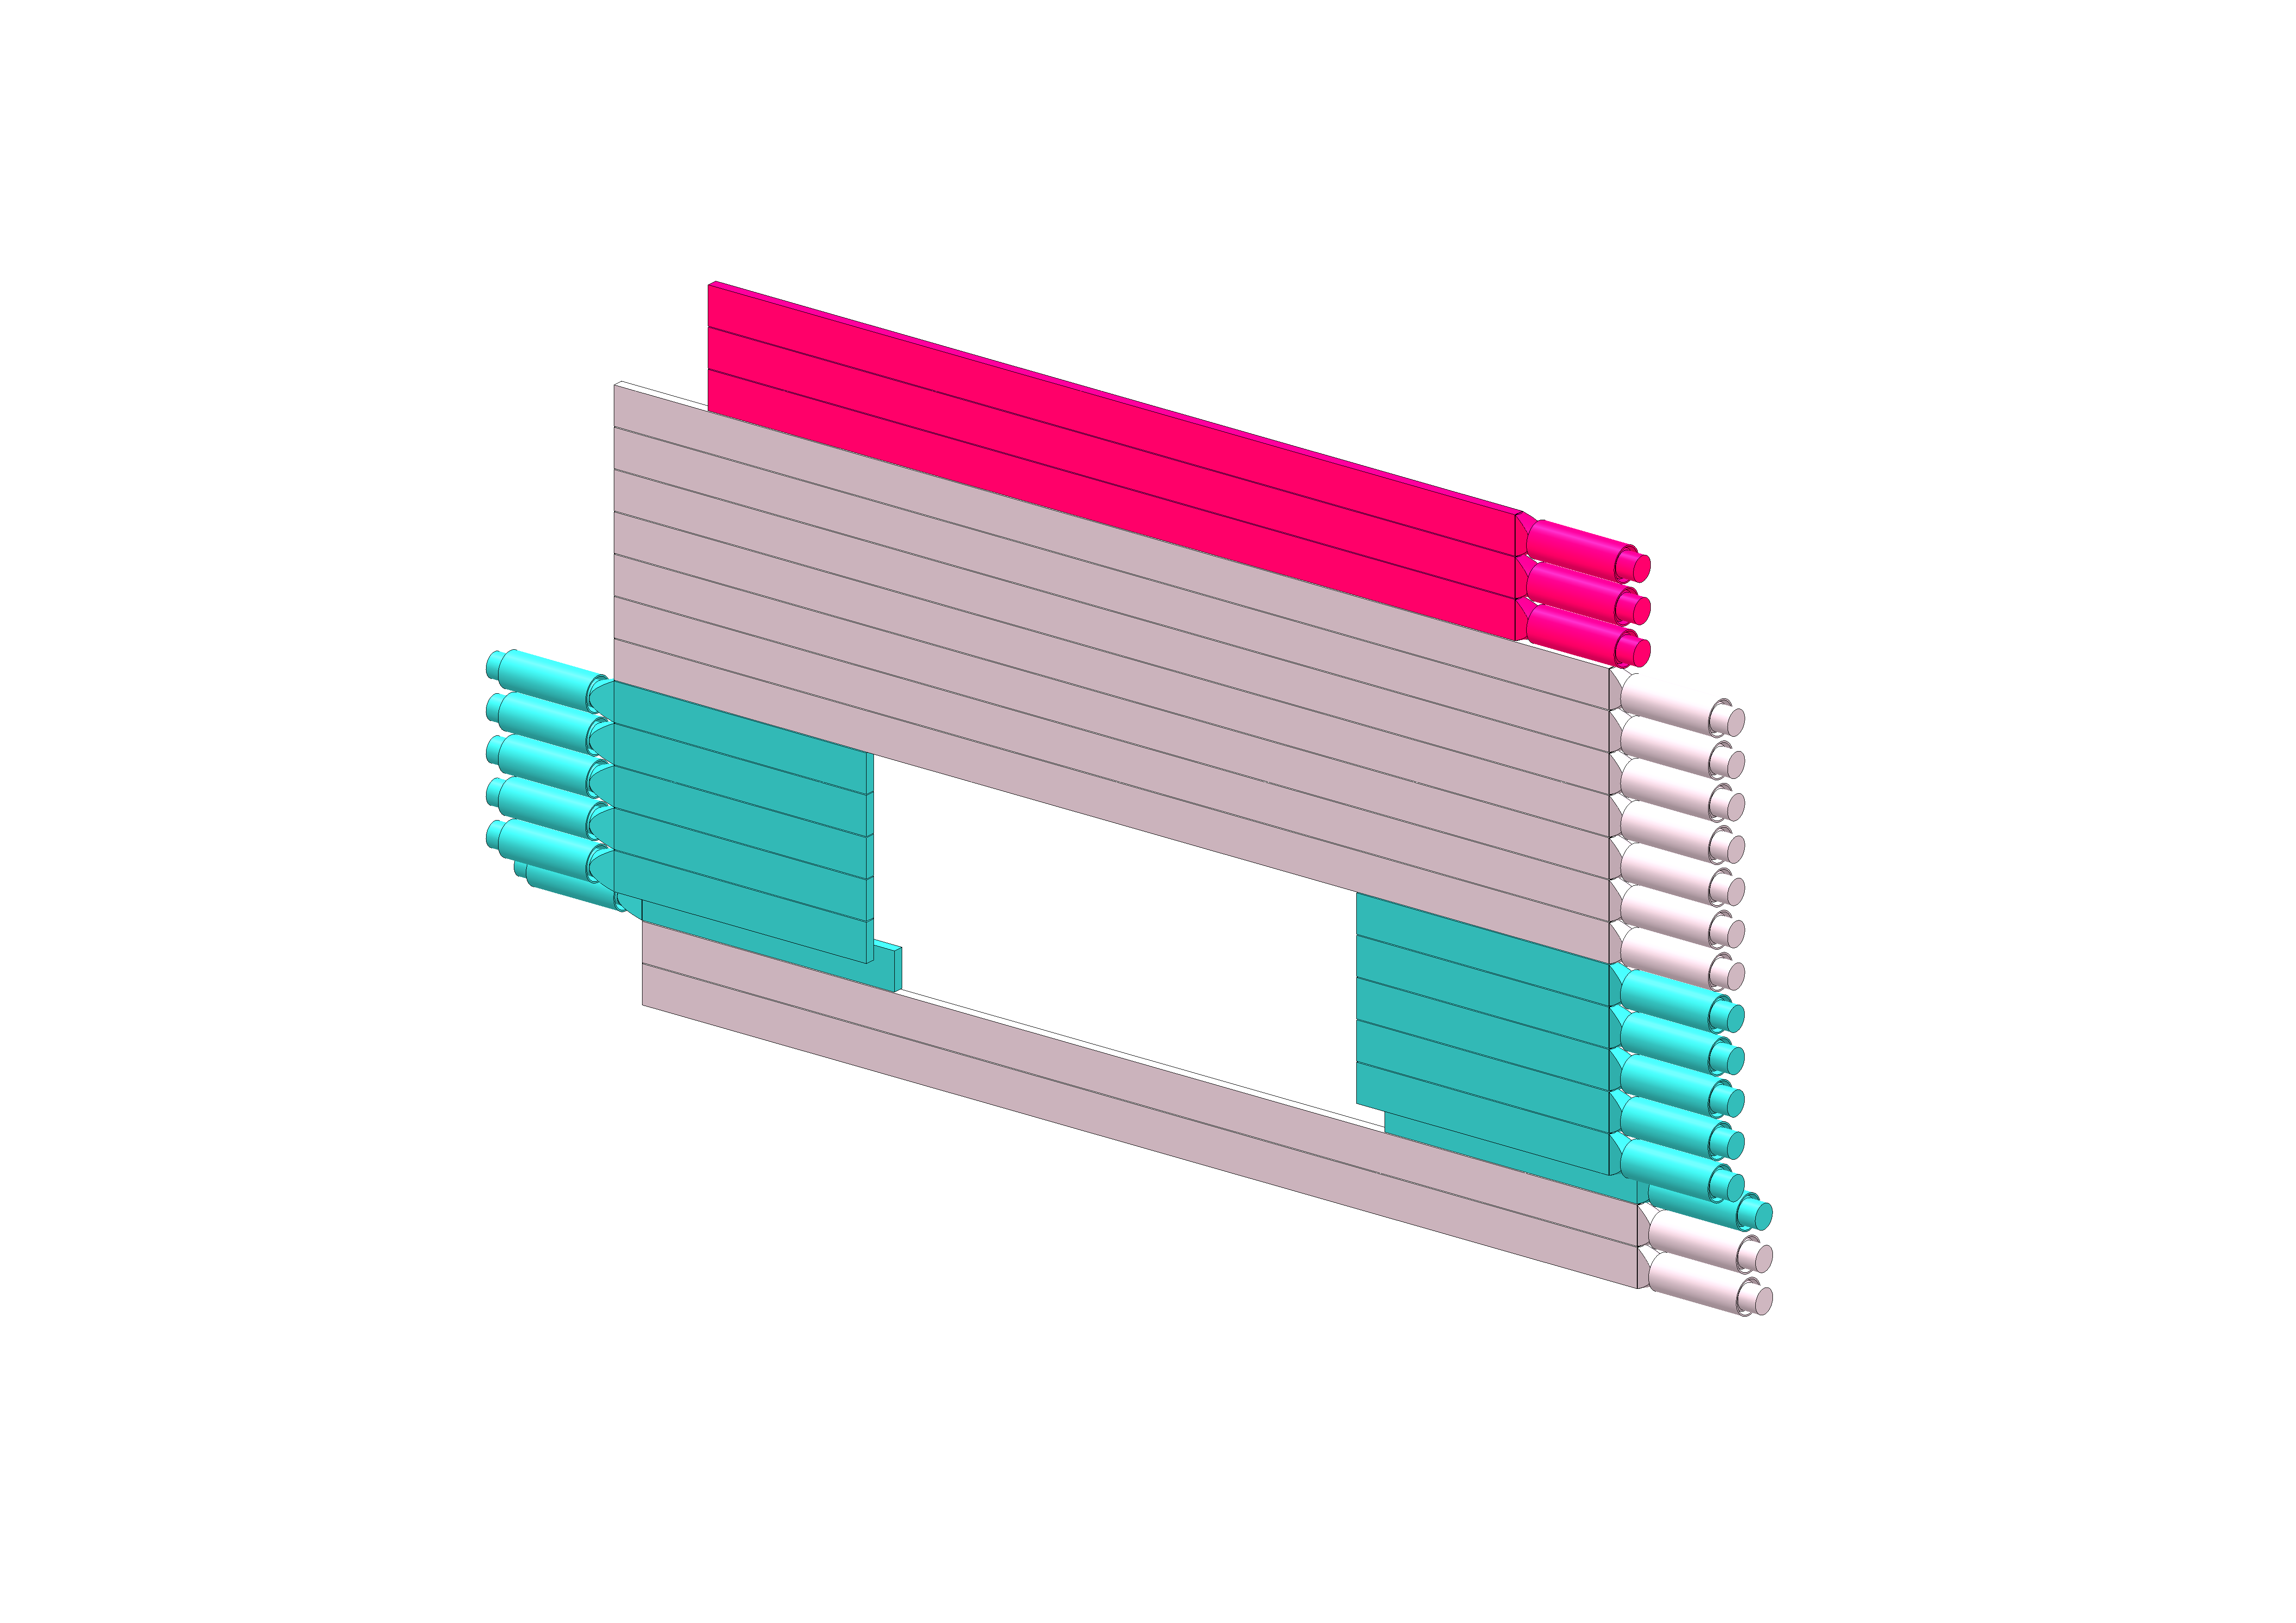
\includegraphics[width=0.48\textwidth]{VETO_DETECTOR_COLORED_2.png}
		\caption{BAND design. Need an updated nicer figure with direction of beam / coordinate system. Also have a similar 
		color scheme denoting the different sectors, so let's do a darker/ligher shade of green for the short bars so we can make 
		a table of sector, layer, ID, etc..}
		\label{fig:design}
\end{figure}

\subsection{Calibration system}
Due to the placement of the BAND, in CEBAF 12 \si{\giga\electronvolt} with the CLAS12 magnetic fields [{\color{red}CITE}], there is a lack of high-rate exclusive processes 
that can be used for monitoring performance stability and perform calibrations. A laser system [{\color{red}CITE}] was implemented to validate performance during data-taking. This system also 
provided a method to quickly perform calibrations (discussed below).

\subsection{Components}
The timing resolution of the scintillator bars is impacted by many factors, and each component was optimized considering the design constraint and cost. Tests were 
performed varying the scintillant, reflective wrapping, photo-multipler tube (PMT), and optical-coupling-method of the scintillators to light-guides to PMTs; see 
Table~\ref{tab:tests} and Fig.~\ref{fig:test_stand}. 

To extract the time resolution of a PMT, we make use of a coincidence signal between a ``test" scintillator bar and a ``reference" scintillator bar. Each bar has 2 PMTs 
coupled to the ends; the test bar has the PMTs which we wish to measure the time resolution. Both bars are wrapped in an optical reflector, and made light-tight 
via use of tape, coverings, and a black-box. The reference bar parameters are never changed during any measurement. 

A $^{60}$Co source is used as a coincidence signal between the two bars. $^{60}$Co undergoes $\beta^-$ decay to an excited state $^{60}$Ni, which then undergoes 
two $\gamma$ decays down to a $0^+$ ground state (1.17, 1.33 MeV respectively). The two $\gamma$-rays being angularly correlated have a preferred back-to-back 
emission of 180$\degree$. The $^{60}$Co source is collimated by two lead bricks to deposit the $\gamma$-rays at specific locations along the bars, allowing for the 
study of PMT time resolution as a function of distance from the PMT (or, due to attenuation along the bar, effective-energy observed by the PMT).

{\color{red}Discuss the results of the test and which PMT was chosen / why.}

\begin{table}[t!]
	\caption{Tested configurations. Resolution given $2$ \si{\mega\electronvolt} energy deposit in middle of bar.}
	\begin{tabular}{  m{5em} | m{4em} | m{5em} | m{4em} | m{3em} |  m{5.7em} | m{3em} }
		\hline
			Scintillator & Reflector & PMT & Optical-coupling & Length (cm) & Cross section (\si{\centi\meter} x \si{\centi\meter}) & $\sigma$ (\si{\pico\second})\\
		\hline
		\hline
			EJ-200 & Al foil & ET-9214 & Grease & 200 & 7 x 7 & 270			\\
		
			EJ-200 & Al foil & R7724-10 & Grease & 200 & 7 x 7 & 240		\\
			EJ-200 & Al foil & R13435 & Grease & 200 & 7 x 7 & 300 			\\
		
			EJ-200 & Al foil & R13089 & Grease & 250 & 5 x 5  & 220			\\
			EJ-200 & Al foil & R7724-100 & Grease & 250 & 5 x 5 & 200 		\\
			
			BC-408 & XXX & ET-9214 & RTV 615 &50 & 7 x 7 & 150				\\
			BC-408 & XXX & R7724-10 & RTV 615 & 200 & 7 x 7 & 150			\\
		\hline
	\end{tabular}
	\label{tab:tests}
\end{table}

\begin{figure}[h!]
	\centering
	\begin{minipage}{0.48\textwidth}
		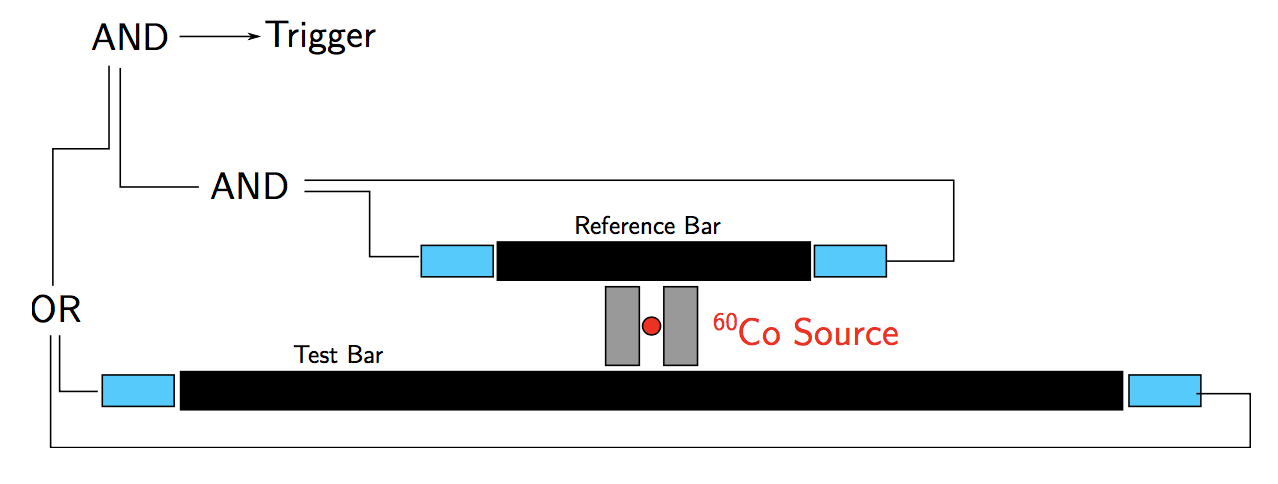
\includegraphics[width=\textwidth]{phys_setup.png} \\
		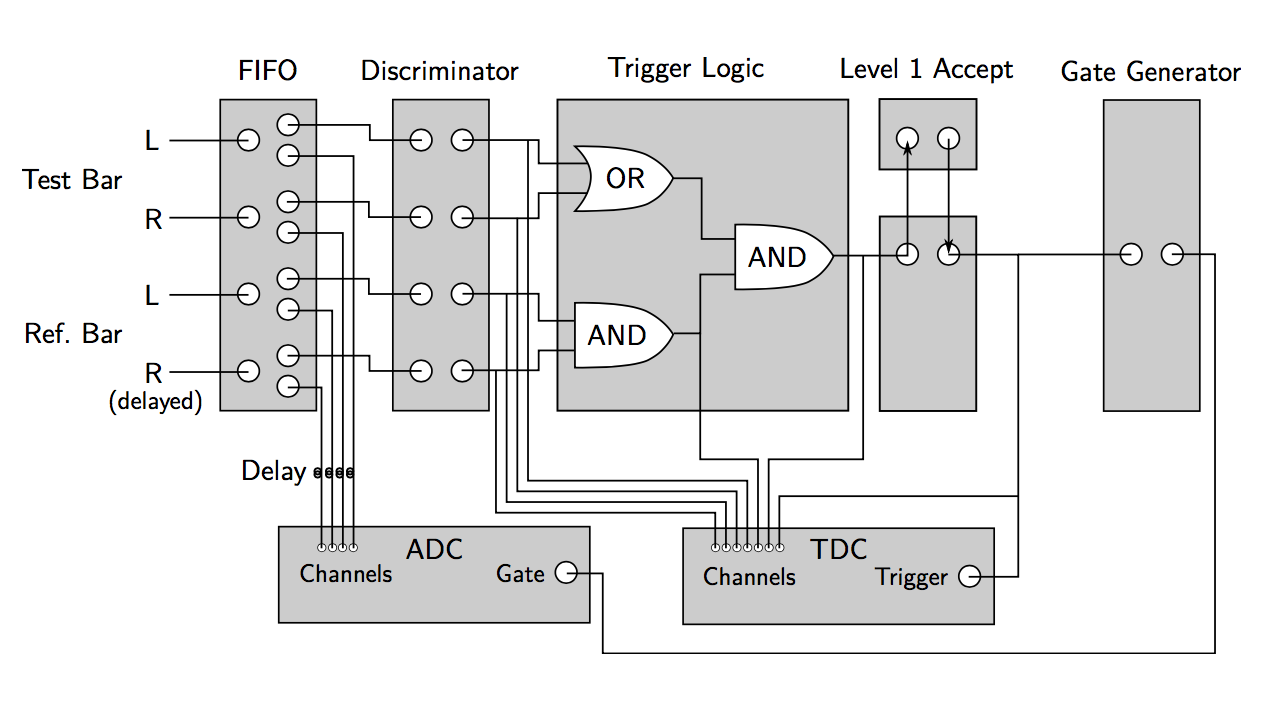
\includegraphics[width=\textwidth]{electr_setup.png}
	\end{minipage}
	\begin{minipage}{0.48\textwidth}
		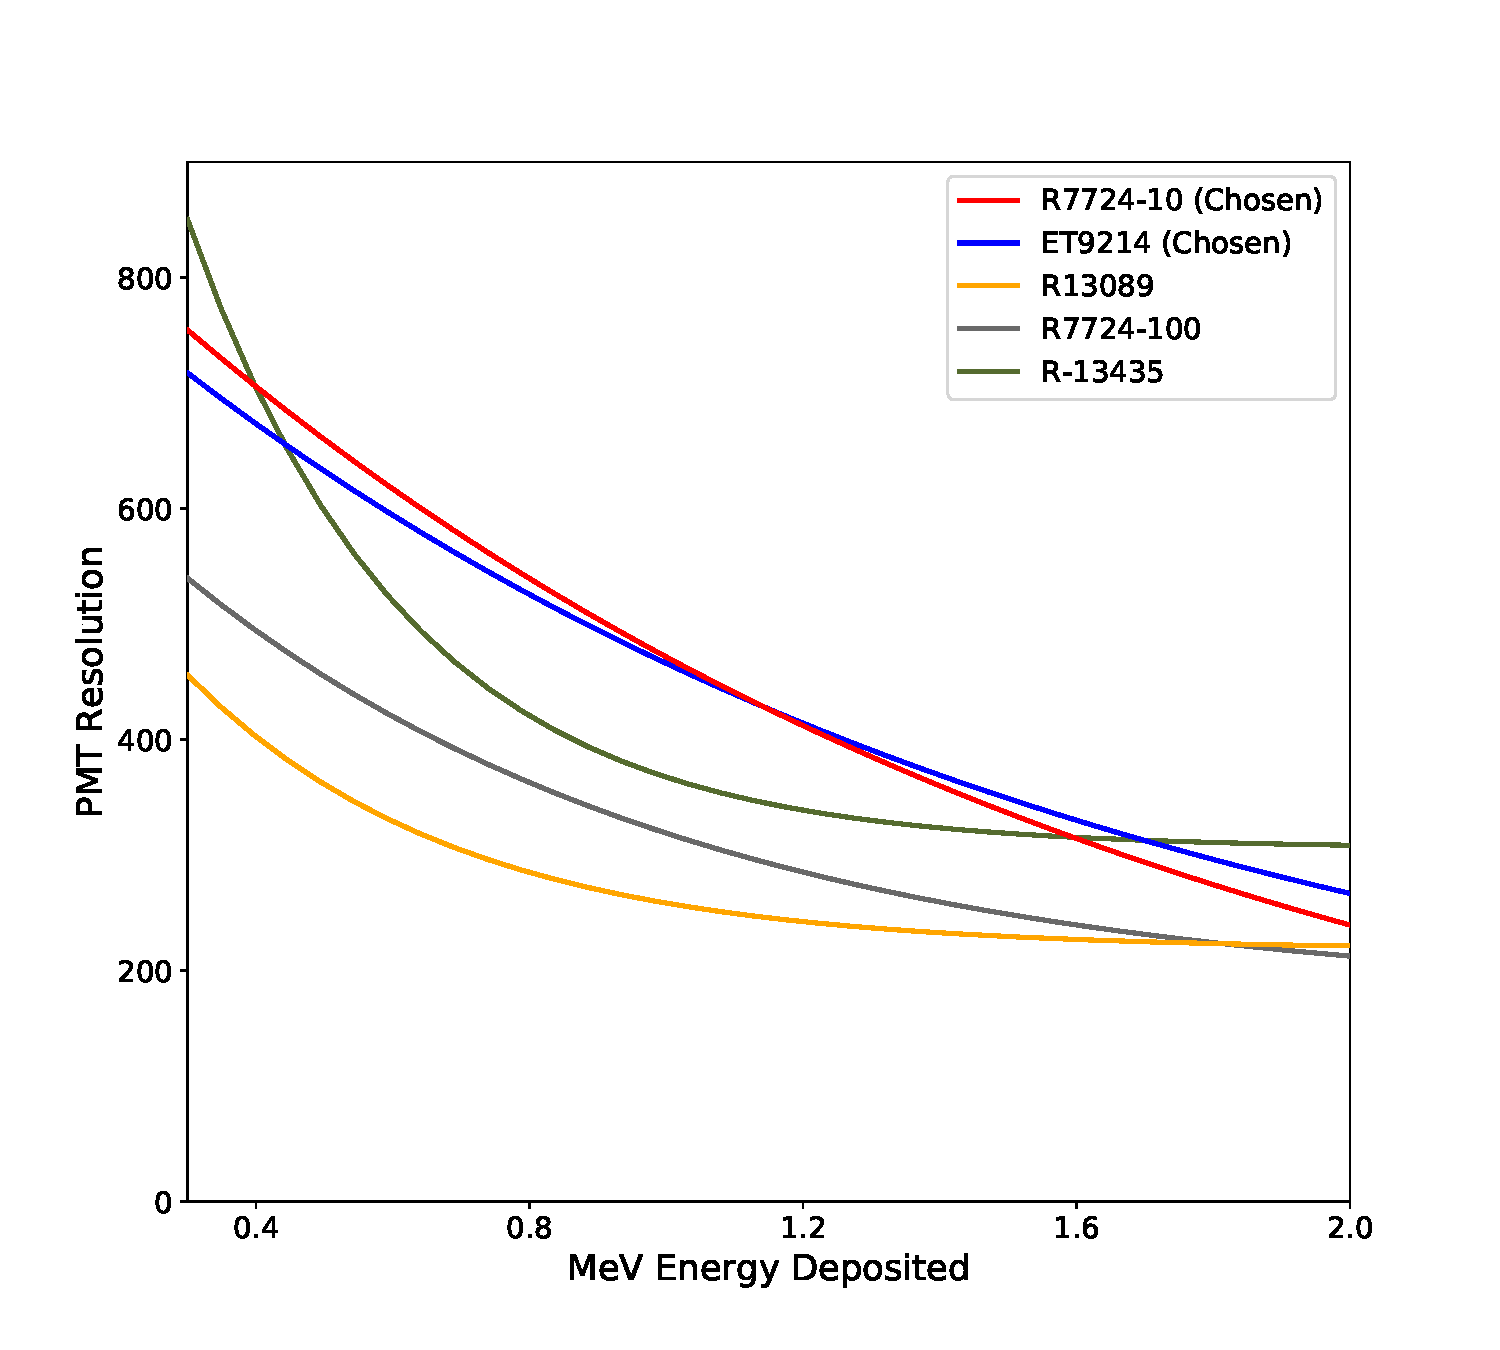
\includegraphics[width=\textwidth]{test-stand/test-resolutions.pdf}
	\end{minipage}
	\caption{Test stand setup and results}
	\label{fig:test_stand}
\end{figure}

\subsection{Magnetic shielding}
{\color{red}EDIT TEXT FROM KITTY:
Magnetic shielding testing for BAND was conducted at ODU. We constructed a pair of 56-turn Helmholtz coils with a radius of 0.5 m, one borrowed from an existing setup, and one welded and wrapped on-site. We built an aluminium frame to maintain coil spacing, and laid a wooden platform between the coils. We also built a small prototype detector consisting of a 2 cm thick, 5 cm diameter disc of plastic scintillant, 7 cm long, 5 cm diameter cylindrical acrylic light guides, and PMTs with voltage dividers of the type we anticipated using to build the final detector. The disc of scintillant was mounted to the light guides with two-part optical cement, and the PMTs were mounted temporarily using optical grease. The detector was then light-proofed with Tedlar and stabilized in a simple cradle of PMT shipping foam. The cradle was placed on a stack of plastic shelving to center it in the field, then covered with black fleece.

As a baseline, the TDC and ADC peaks produced by strontium-90 and caesium-137 sources, and two different source placements were measured for a nominal operating voltage of the PMTs with no shielding. The goal was to place shielding such that the fewest number of events would be lost and the effect on timing would be minimized as magnetic field increased.

We tested two thicknesses of mu-metal shielding, each in two diameters, as well as two pipes of soft iron. The magnetic field, amount of detector covered by the shielding, the thickness of the shielding, the placement of two radioactive sources, and the angle of the detector to the field were all varied. The following table shows the full complement of variables:

*only the caesium-137 was tested at 5 cm. The strontium-90 source triggered too few events when not directly atop the detector.

Magnetic field: varied by changing current in the coils, limited to 80 gauss to prevent melting
Angle: changed by aligning PMT cradle with markers on the magnet platform
Cover: measured from PMT face, along light guides
Shield thickness: varied by sliding one or both thicknesses of mu-metal shielding over the PMTs. Soft iron was only tested alone.
--------

We concluded that (***I forget what thickness was finally ordered...***) mu-metal shielding placed 5 cm past the PMT faces was most effective to preserve events and minimize timing distortions.
}

\subsection{Lead shielding}
{\color{red}Why did we end up putting lead shielding - just a guess?}

%%%%%%%%%%%%%%%%%%%%%%%%%%%%%%%%%%%%%%%%%%%%%%%%%%%%%%%%%%%%%%%%%%%%%%%%%%%%%%%%%%%%%%%%%%%%%%%%%%%

\section{Description}

%%% ----------------- Geometry subsection
\subsection{Geometry}

%%% ----------------- Components subsection
\subsection{Components}

%\begin{table}[t!]
%	\caption{}

%	\label{tab:tests}
%\end{table}


%%% ----------------- Assembly subsection
\subsection{Assembly}

%%% ----------------- Electronics subsection
\subsection{Electronics}
In order to operate the PMTs, high voltages (typically in the range of 1500 V) are provided by a multi-channel CAEN SYS4527 mainframe with 11 A1535SN cards (24 channel each).
The signal of each PMT is sent to an splitter. The splitter are the same as the one used by the HPS experiment.
From the splitter one signal is sent to flash-ADCs (250 VXS, 16 channels/board, made and owned by JLab) while the other signal is sent to  discriminators used by HPS (16 channels/board).
The discriminated time signal then goes to a TDC (CAEN VX1190A, 128 channels/board, 100 ps/channel resolution). The read-out system is installed left of BAND in beam direction. 
In total, the system consists of 16 flash-ADCs in one VXS crate, 16 discriminators and a TDC in a VME crate and 16 splitters.  Furthermore, a signal distribution card for the flash-ADCs and trigger interface boards are installed in the crates. A trigger for cosmics for testing and on a pulser for the laser calibration system will be implemented. BAND does not need to be implemented in the main event triggers of CLAS12.

\begin{figure}[h!]
	\centering
		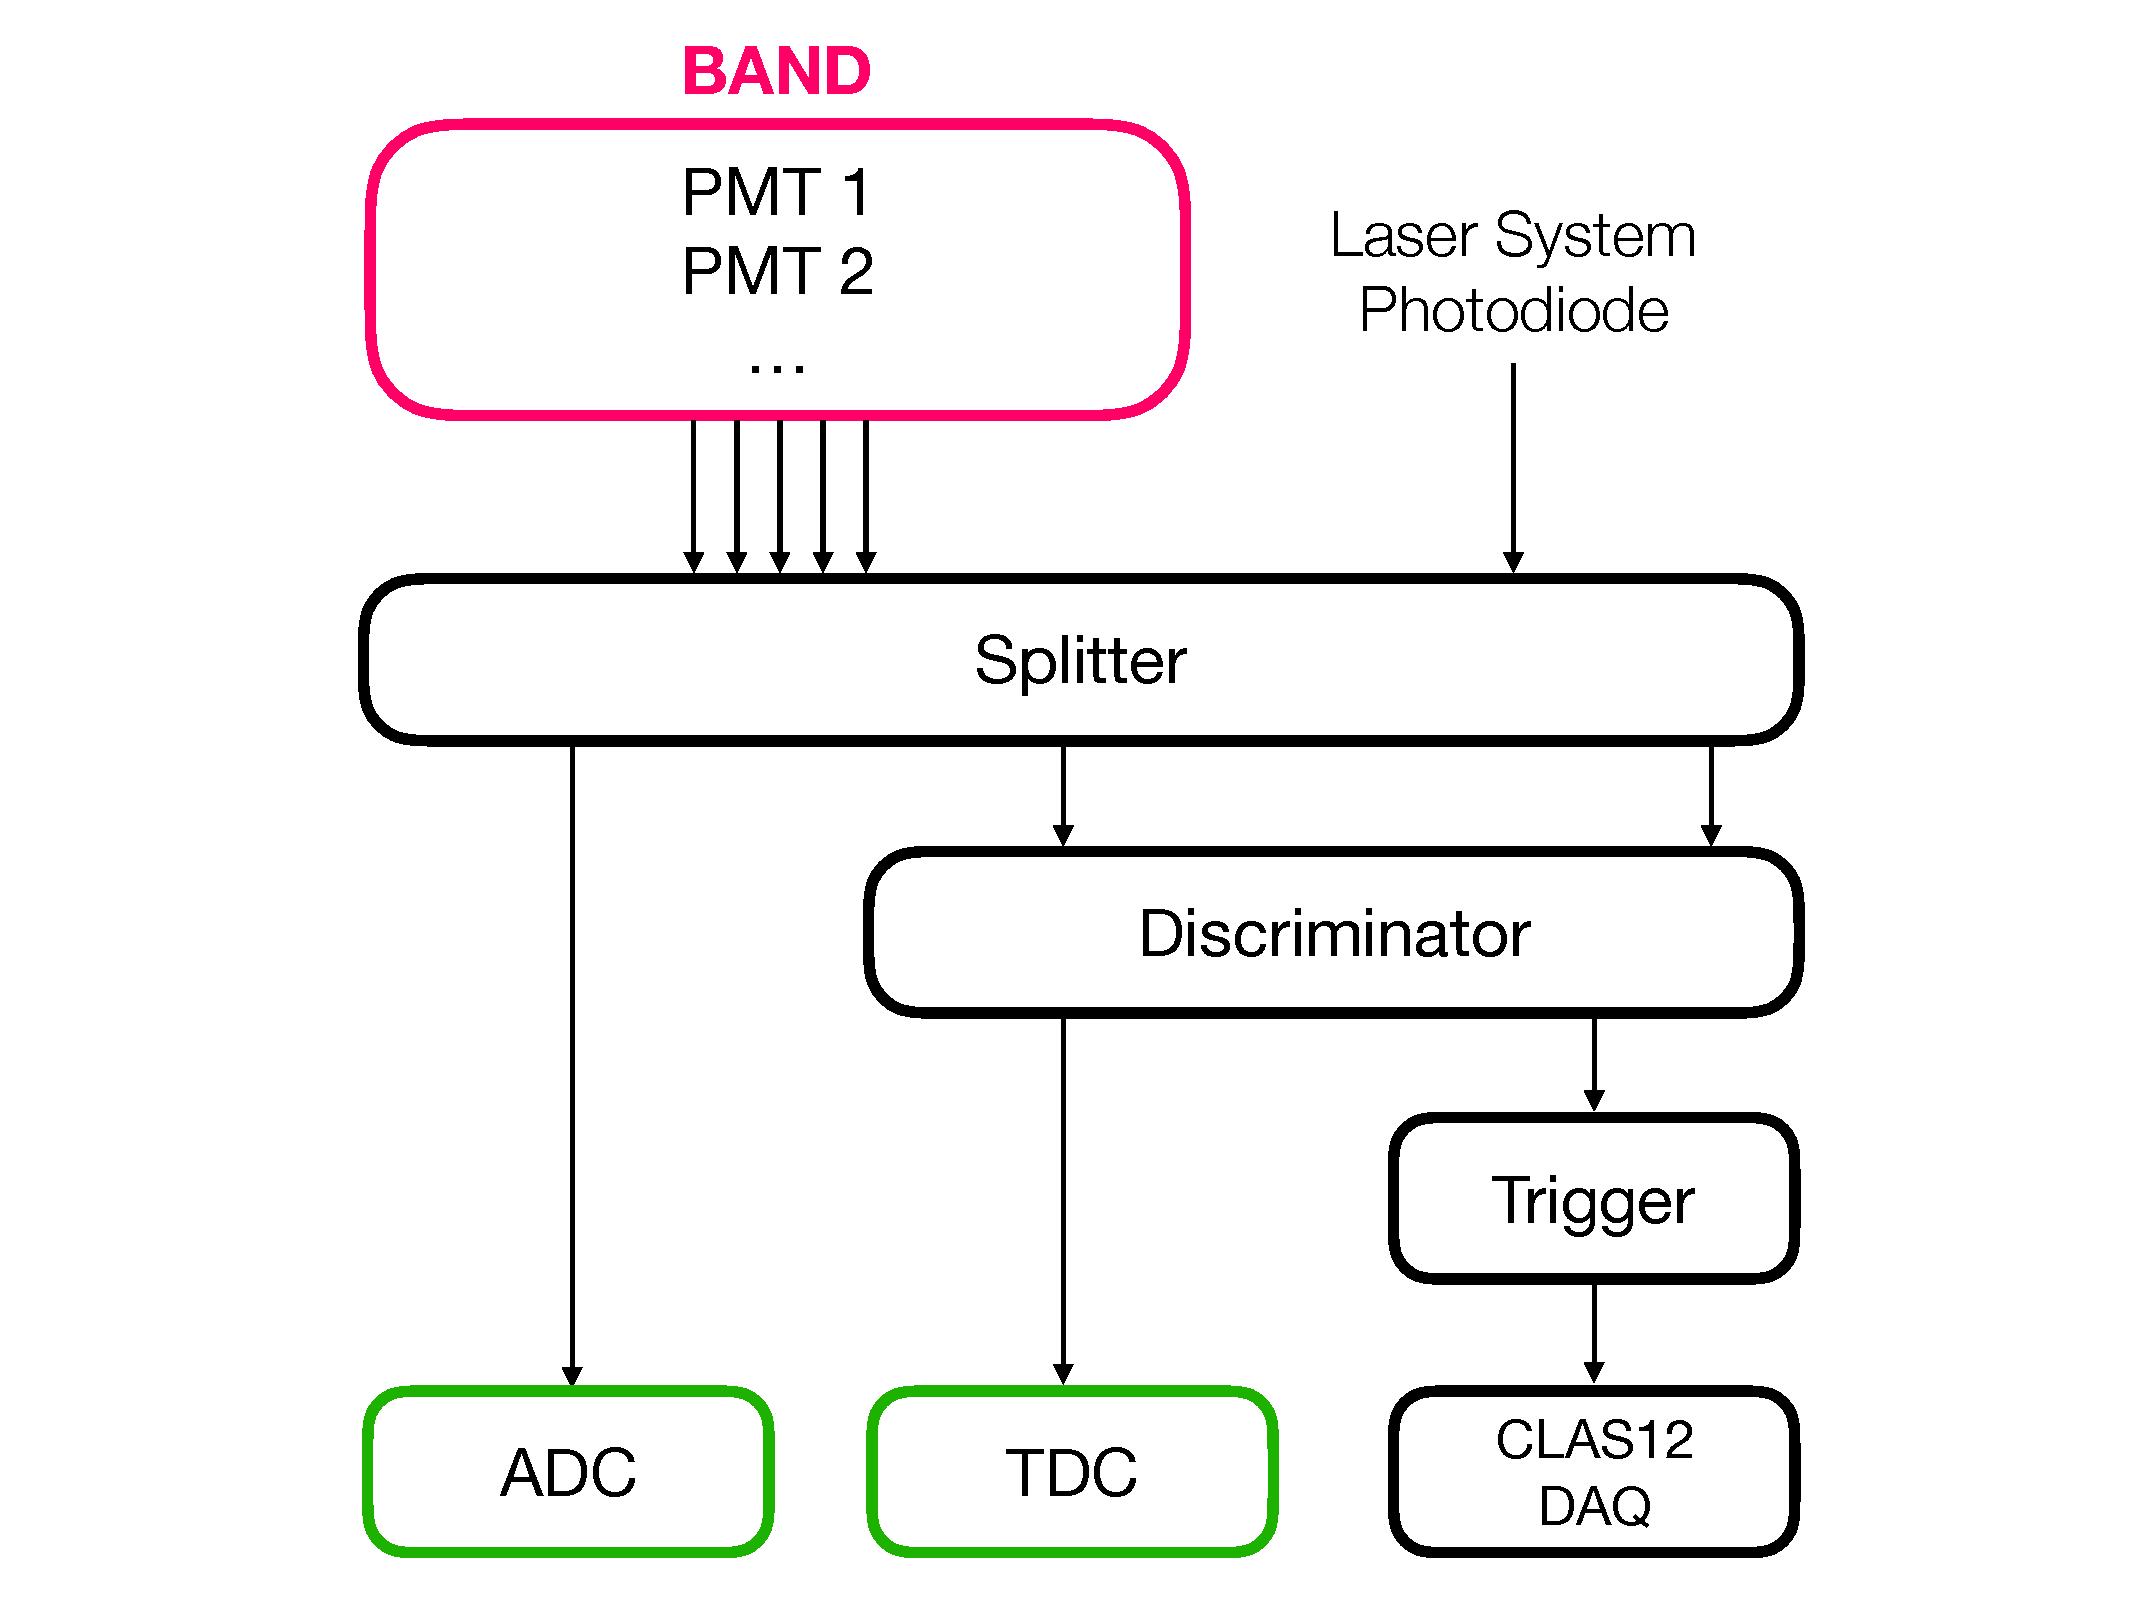
\includegraphics[width=0.96\textwidth]{figures/electronics-diag.pdf}
	\caption{Electronic schematic for }
	\label{fig:electronic-diag}
\end{figure}

%%% ----------------- Laser system subsection
\subsection{Laser calibration system}

%%%%%%%%%%%%%%%%%%%%%%%%%%%%%%%%%%%%%%%%%%%%%%%%%%%%%%%%%%%%%%%%%%%%%%%%%%%%%%%%%%%%%%%%%%%%%%%%%%%


\section{Performance}
%%% ----------------- Gain matching subsection
\subsection{Individual bar performance}
\subsubsection{Gain matching}
{\color{red}Could go into much more detail like FTOF does -- what value for cosmic did we match to / why...}
In order to have similar response to a given energy deposit across all PMTs of BAND, each PMT's HV was optimized using
cosmic rays. Multiple data sets with varying PMT HV were taken with cosmic rays, and combined to produce a gain curve for 
each PMT. A typical pulse height spectrum from cosmic data for a single HV setting and the resulting gain curve from fitting the 
cosmic peak from many HV settings are both shown in Fig~\ref{fig:hv_settings}. The resulting HV settings across all PMTs in BAND is 
shown in Fig~\ref{fig:hv_settings}.
\begin{figure}[h!]
	\centering
		\begin{minipage}{0.48\textwidth}
			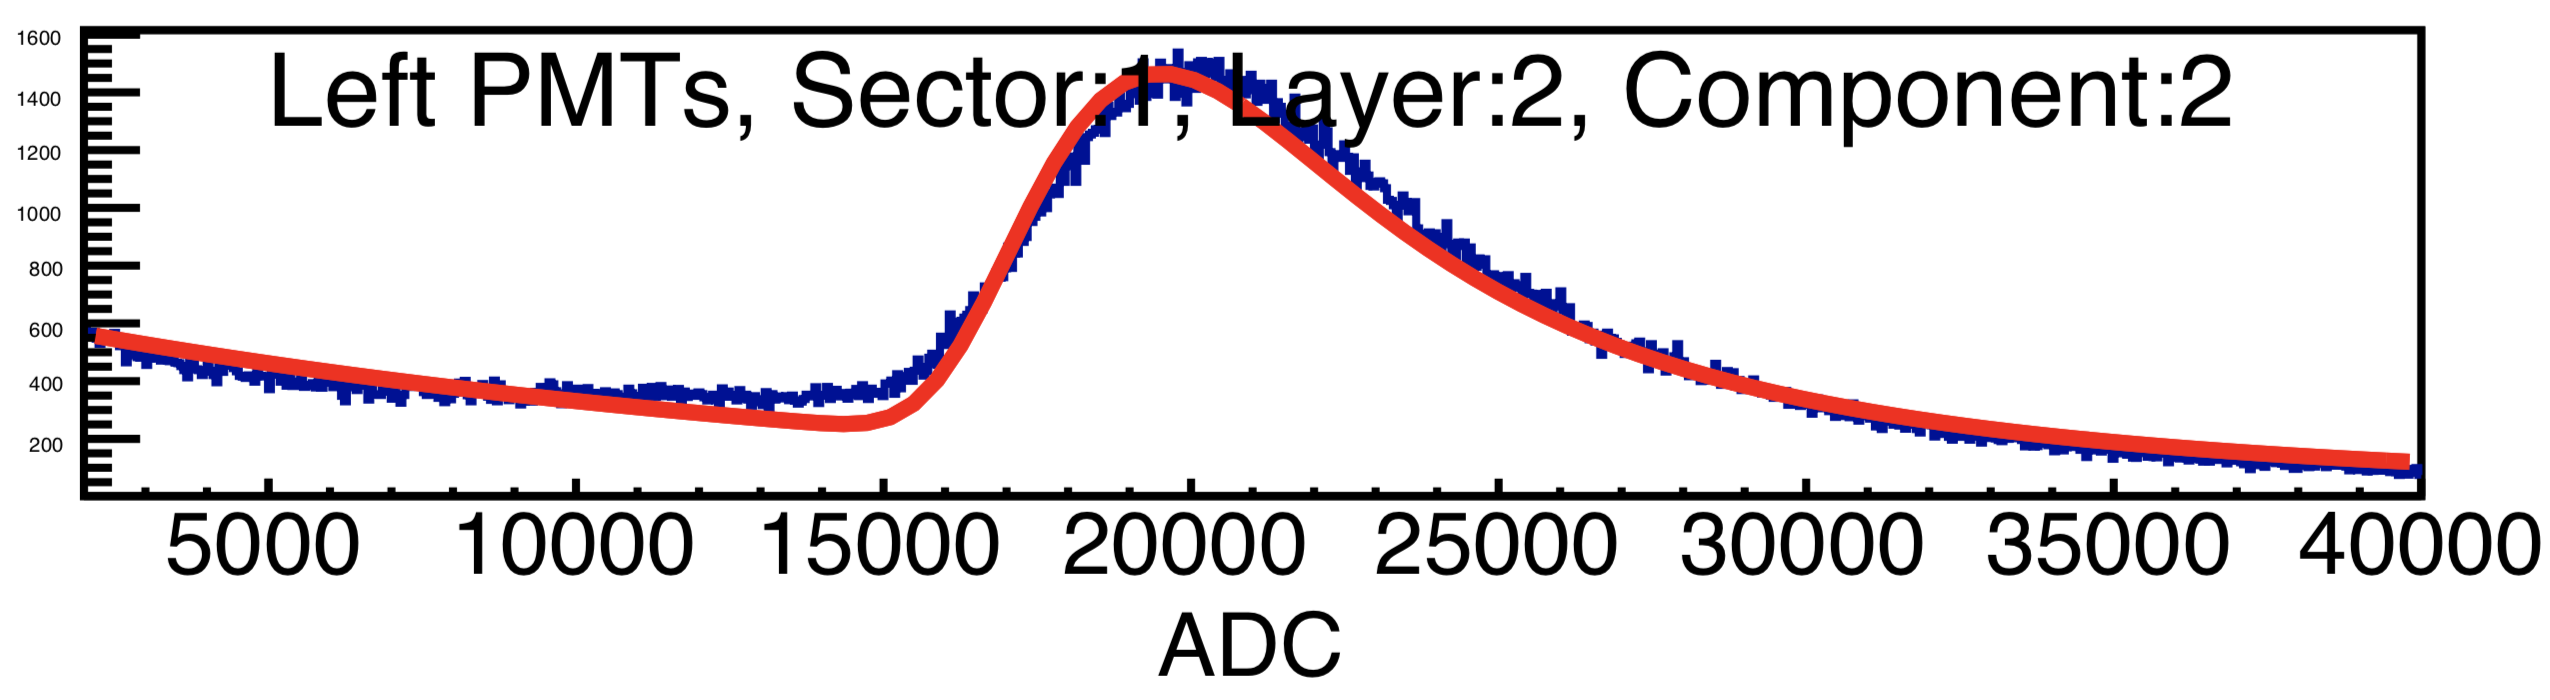
\includegraphics[width=\textwidth]{adc-spectra.png}\\
			%\includegraphics[width=\textwidth]{.png}
			\label{fig:gain}
		\end{minipage}
		\begin{minipage}{0.48\textwidth}
			\includegraphics[width=\textwidth]{hv-settings.pdf}
		\end{minipage}
		
		\caption{Left: pulse height spectrum. Right: gain curve. All PMT HV settings. One sees a greater 
		spread of HV needed to match PMTs in the ET9214 models.}
		\label{fig:hv_settings}
\end{figure}


%%% ----------------- Energy deposit subsection
\subsubsection{Energy deposit calibration}
The ADC response of each PMT is converted to \si{\mega\electronvolt} energy deposition by measuring the response to 
multiple radioactive sources. The sources $^{60}$Co, $^{22}$Na, $^{137}$Cs were chosen due to the gamma rays that have 
Compton edges of $0.963$ and $1.118$, $0.477$, and, $1.062$ and $0.341$, respectively (in \si{\mega\electronvolt}). The 
response to each source was measured in the center of the bar. Using the ADC response to all sources, in combination with the 
attenuation length of the bar, the ADC response can be converted to \si{\mega\electronvolt}.

A typical response of a PMT to  $^{60}$Co is shown in Fig.~\ref{fig:mev_conversion}, along with the extracted Compton edge for a 
number of bars. {\color{red}A lot more detail should be given -- the fact that we do geometric mean of ADC, not done per PMT, etc.. }

\begin{figure}[h!]
	\centering
		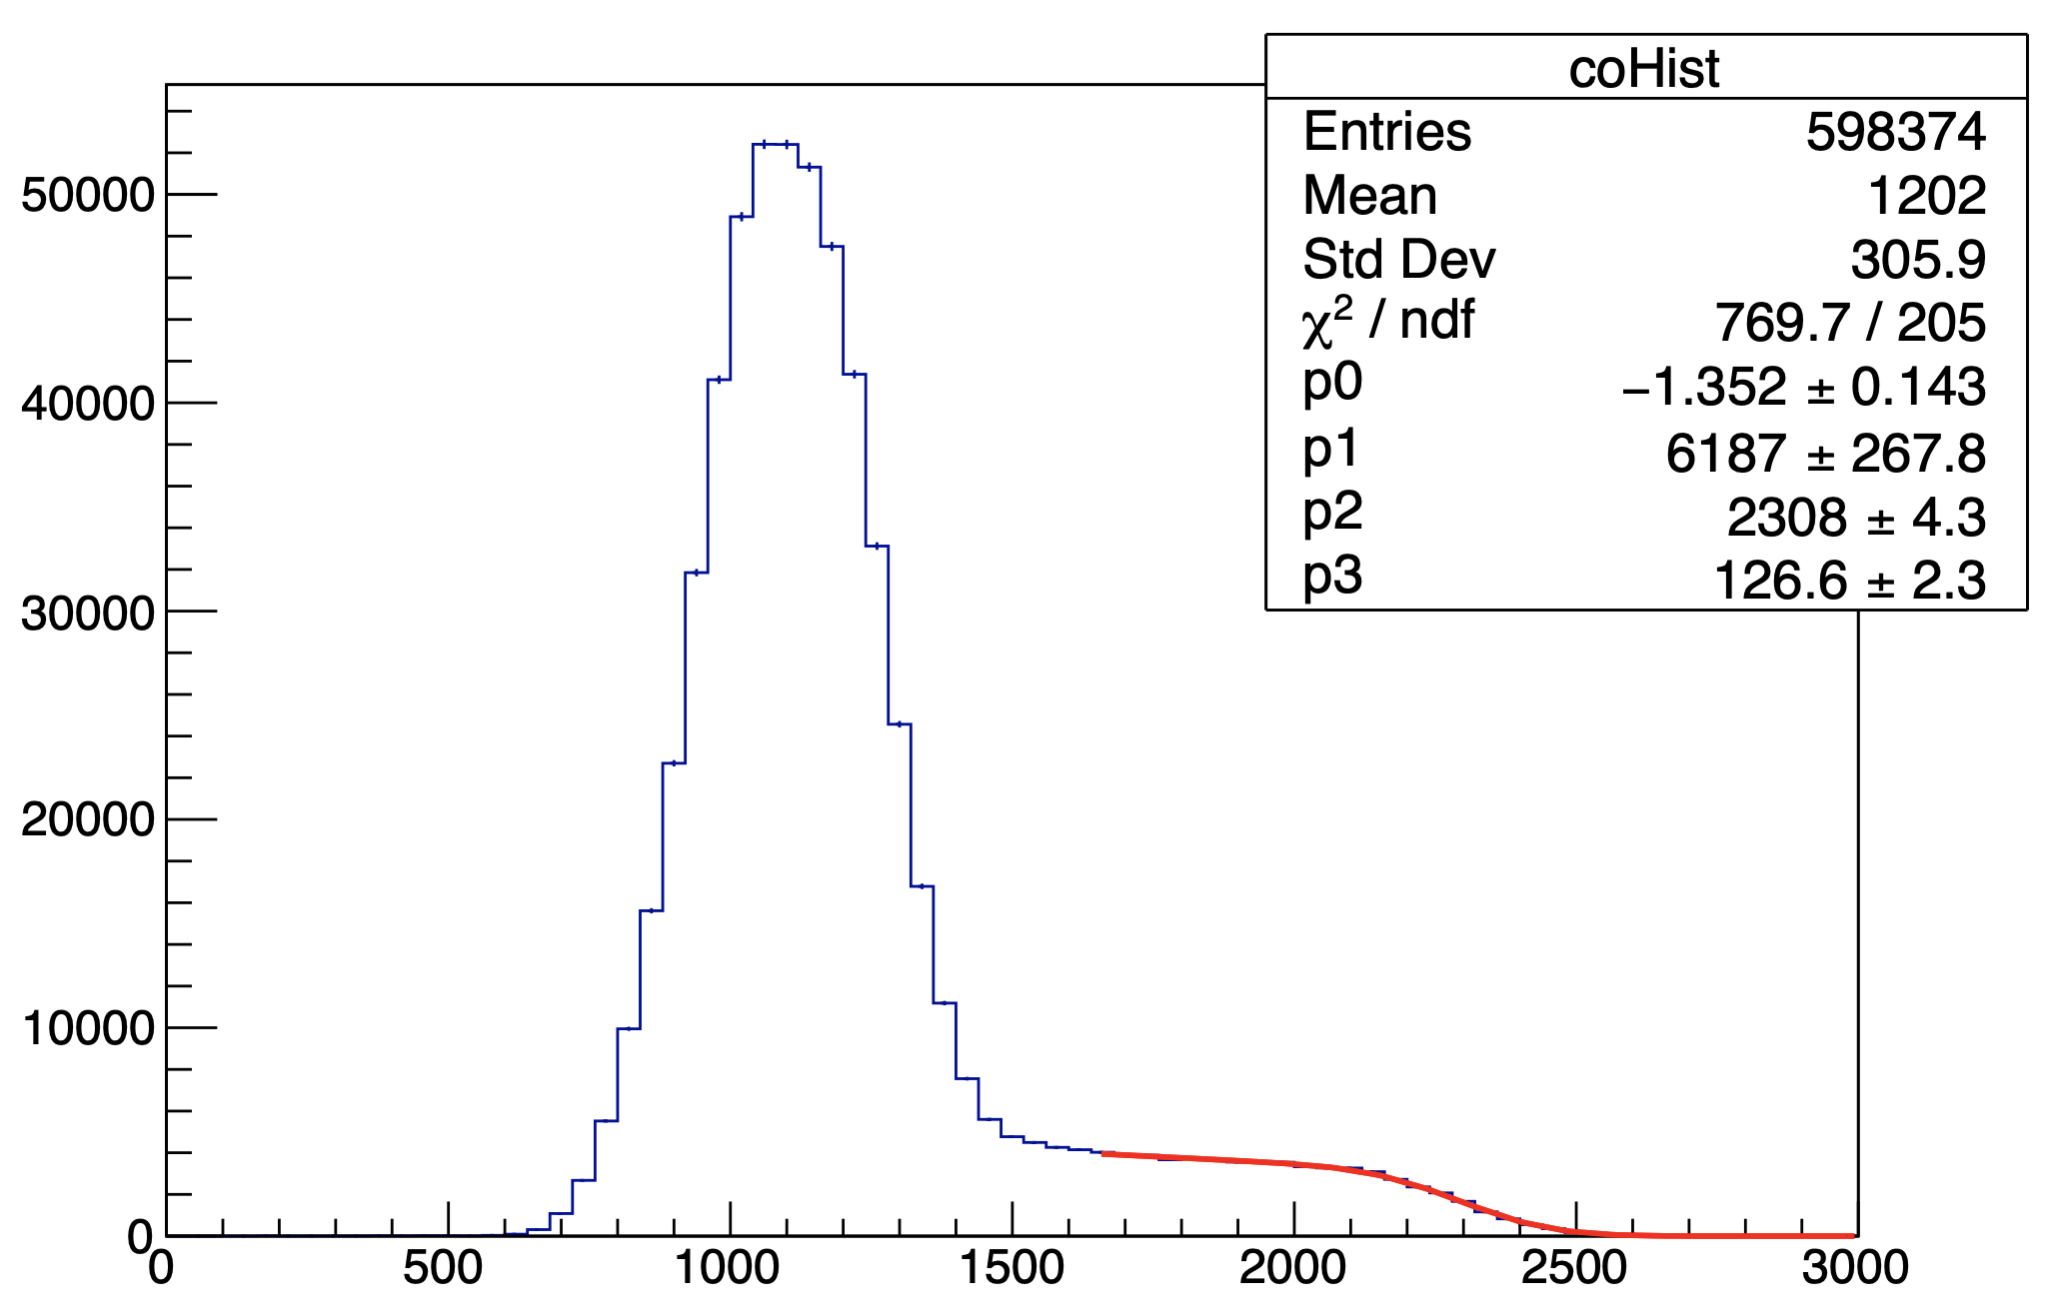
\includegraphics[width=0.48\textwidth]{co-compton.png}
		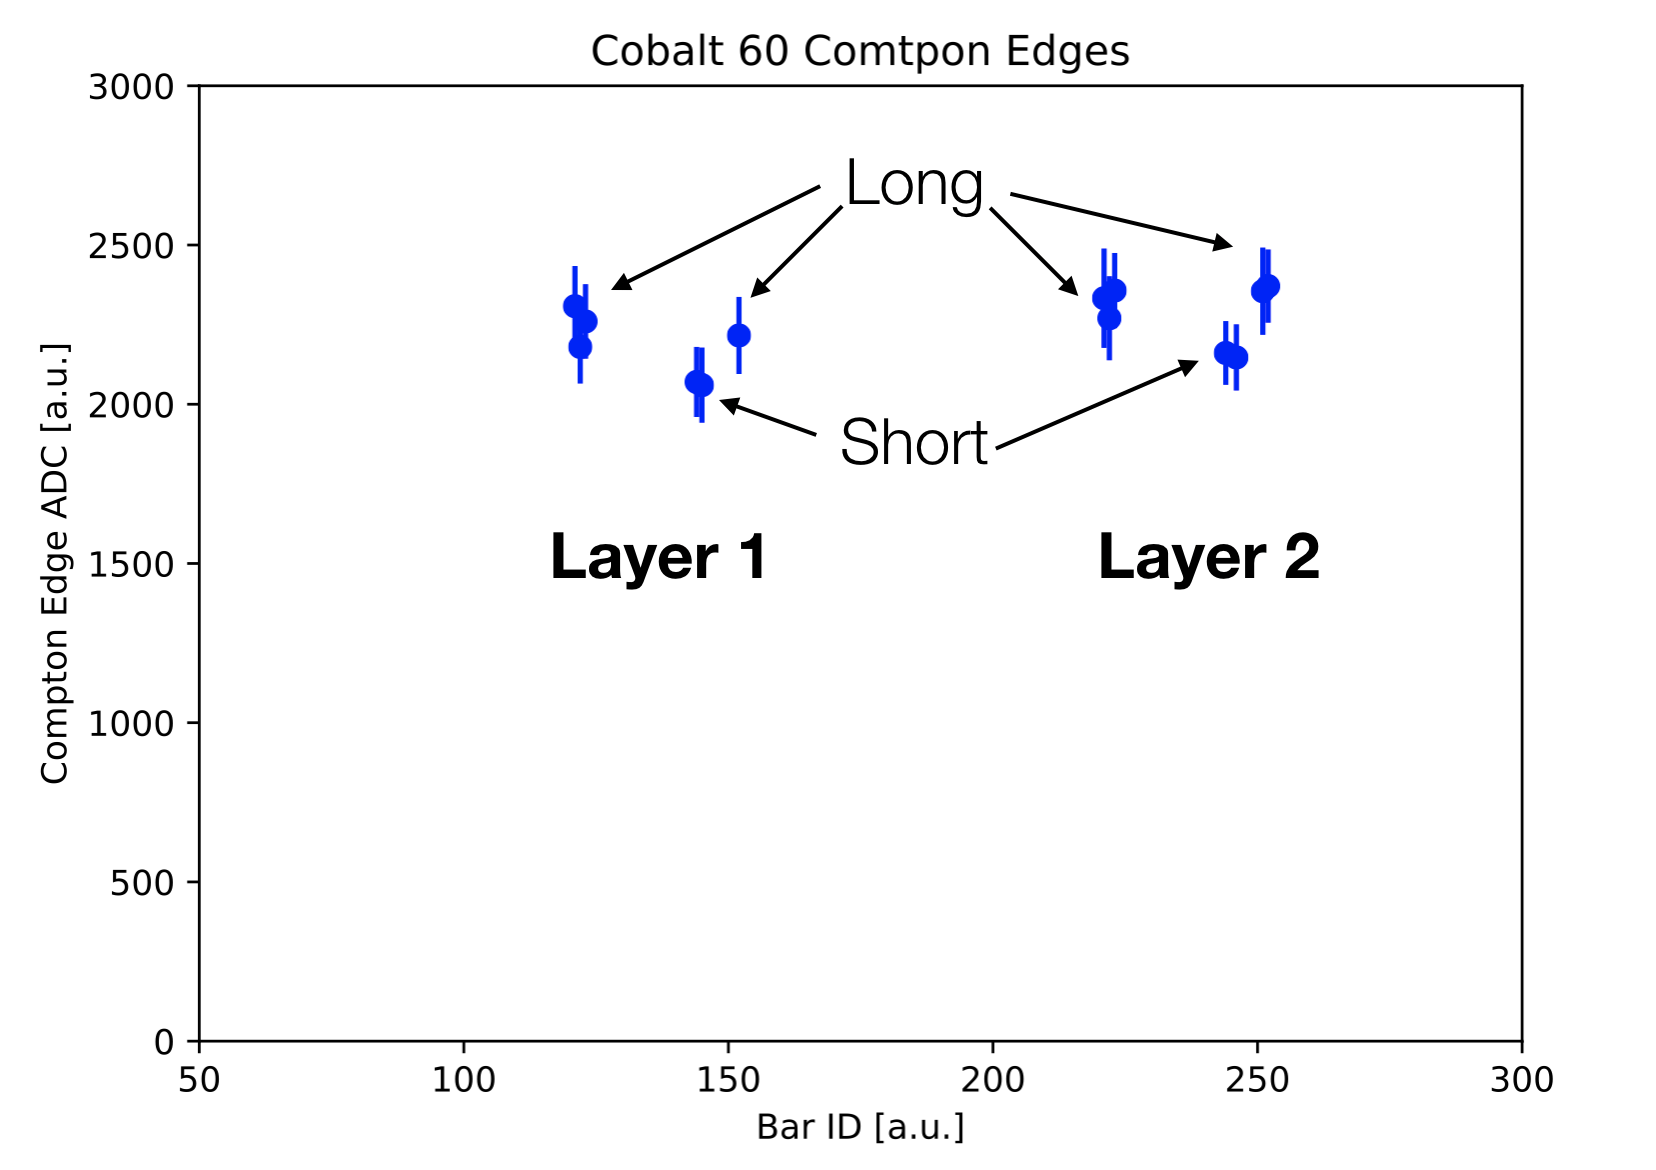
\includegraphics[width=0.48\textwidth]{coedges.png}
	\caption{{\color{red}also need a plot of the 3 sources and their edges to a fit for the conversion}}
	\label{fig:mev_conversion}
\end{figure}

%%% ----------------- Time-walk subsection
\subsubsection{Time-walk calibration}
Time-walk calibrations were performed with the laser system [{\color{red}{CITE}}]. A motorized fiber optic attenuator is used to vary
the amount of light delivered to each bar. Waveforms and times are measured as the attenuator scans from $40$ \si{\decibel} to $0$ 
\si{\decibel}. Time-walk curves and calibrations are taken per PMT. The laser pulse, immediately after fiber-coupling, is initially 
split with $90\%$ going to the attenuator, and $10\%$ going to a photodiode used as a reference time for any calibrations 
performed with the laser system.

Dependence of a typical PMT time to pulse height is seen in Fig.~\ref{fig:time_walk} (left). To correct for time-walk, we parameterize 
this dependence on pulse height, $A$, as:
\begin{eqnarray}
	\begin{split}
		t_*(A)	&= \alpha + \frac{\beta}{\sqrt{\textrm{A}}}.				
		\label{eqn:time_walk}
	\end{split}
\end{eqnarray}
The residual after time-walk correction, $t-t_*$, is shown in Fig.~\ref{fig:time_walk} (right). At pulse heights close to threshold, the 
parameterization is not flexible enough and under-estimates the strong dependence on pulse height. However, signals with pulse 
heights this low are not of interest, as a software cut on minimum energy deposition is needed to improve signal-to-background 
which removes these pulses (discussed in Section {\color{red}4.2.3}).

\begin{figure}[h!]
	\centering
		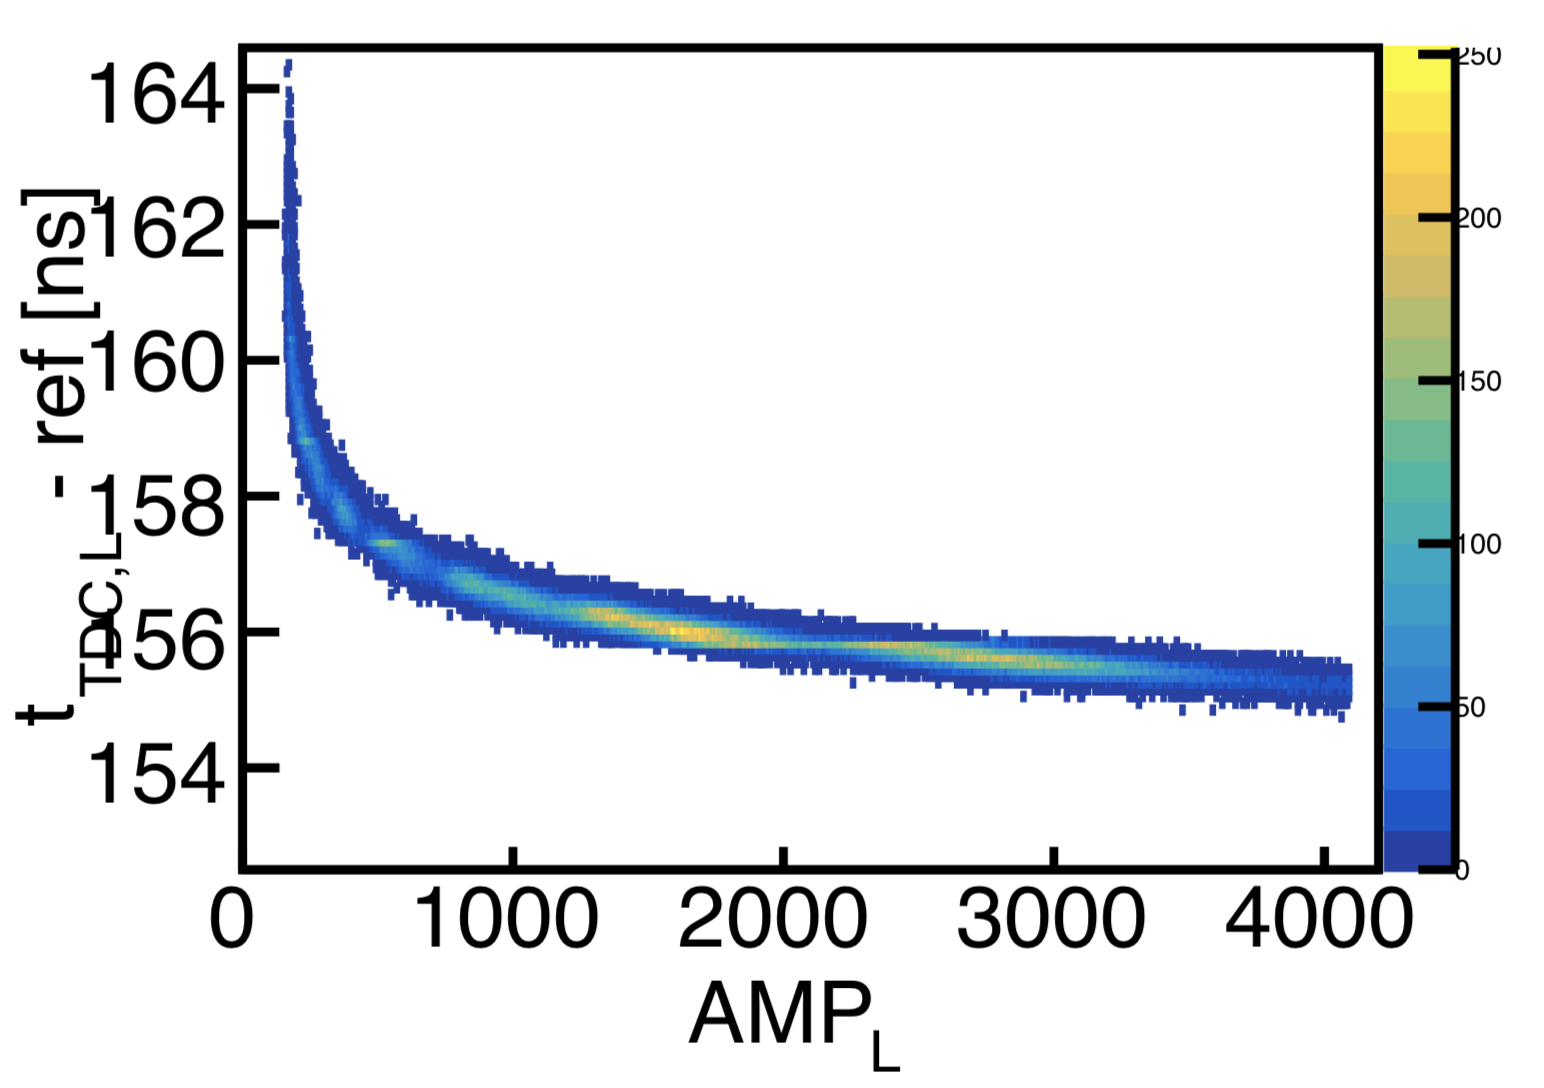
\includegraphics[width=0.48\textwidth]{tw_before.png}
		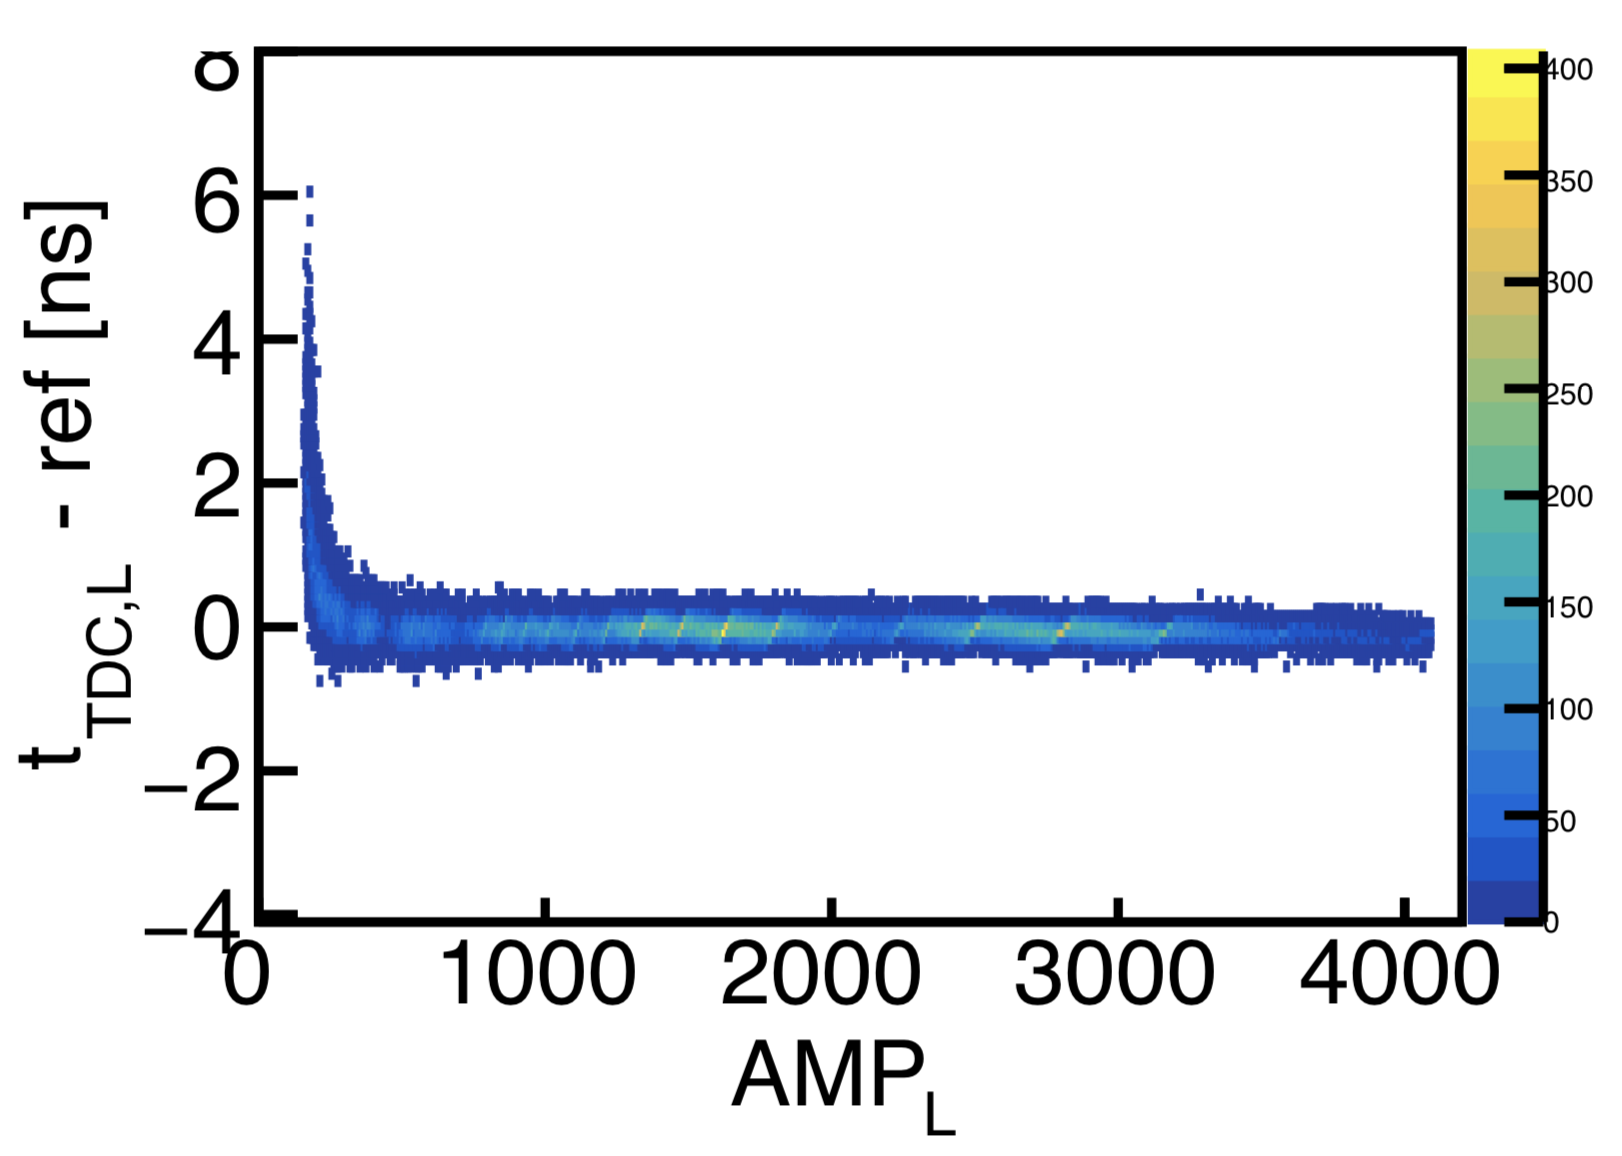
\includegraphics[width=0.48\textwidth]{tw_after.png}
	\caption{}
	\label{fig:time_walk}
\end{figure}

%%% ----------------- Effective velocity subsection
\subsubsection{Effective velocity}
The relative time delays between PMTs on the same bar, and the speed-of-light in that bar, are extracted using cosmic ray 
data after time-walk calibrations are done for each PMT. The width of the relative timing distribution between the left and 
right PMT on a given bar is used to extract the effective velocity in a bar knowing the length of the bar,
\begin{eqnarray}
	\begin{split}
		t_L - t_R 	= -\frac{2x}{v}							\\
		 -\frac{L}{v}	\leq 	t_L - t_R 	\leq \frac{L}{v},				
		 \label{eqn:time_walk}
	\end{split}
\end{eqnarray}

and the relative time offset is given by the center of the distribution. See Fig.~\ref{fig:eff_vel}.

\begin{figure}[h!]
	\centering
		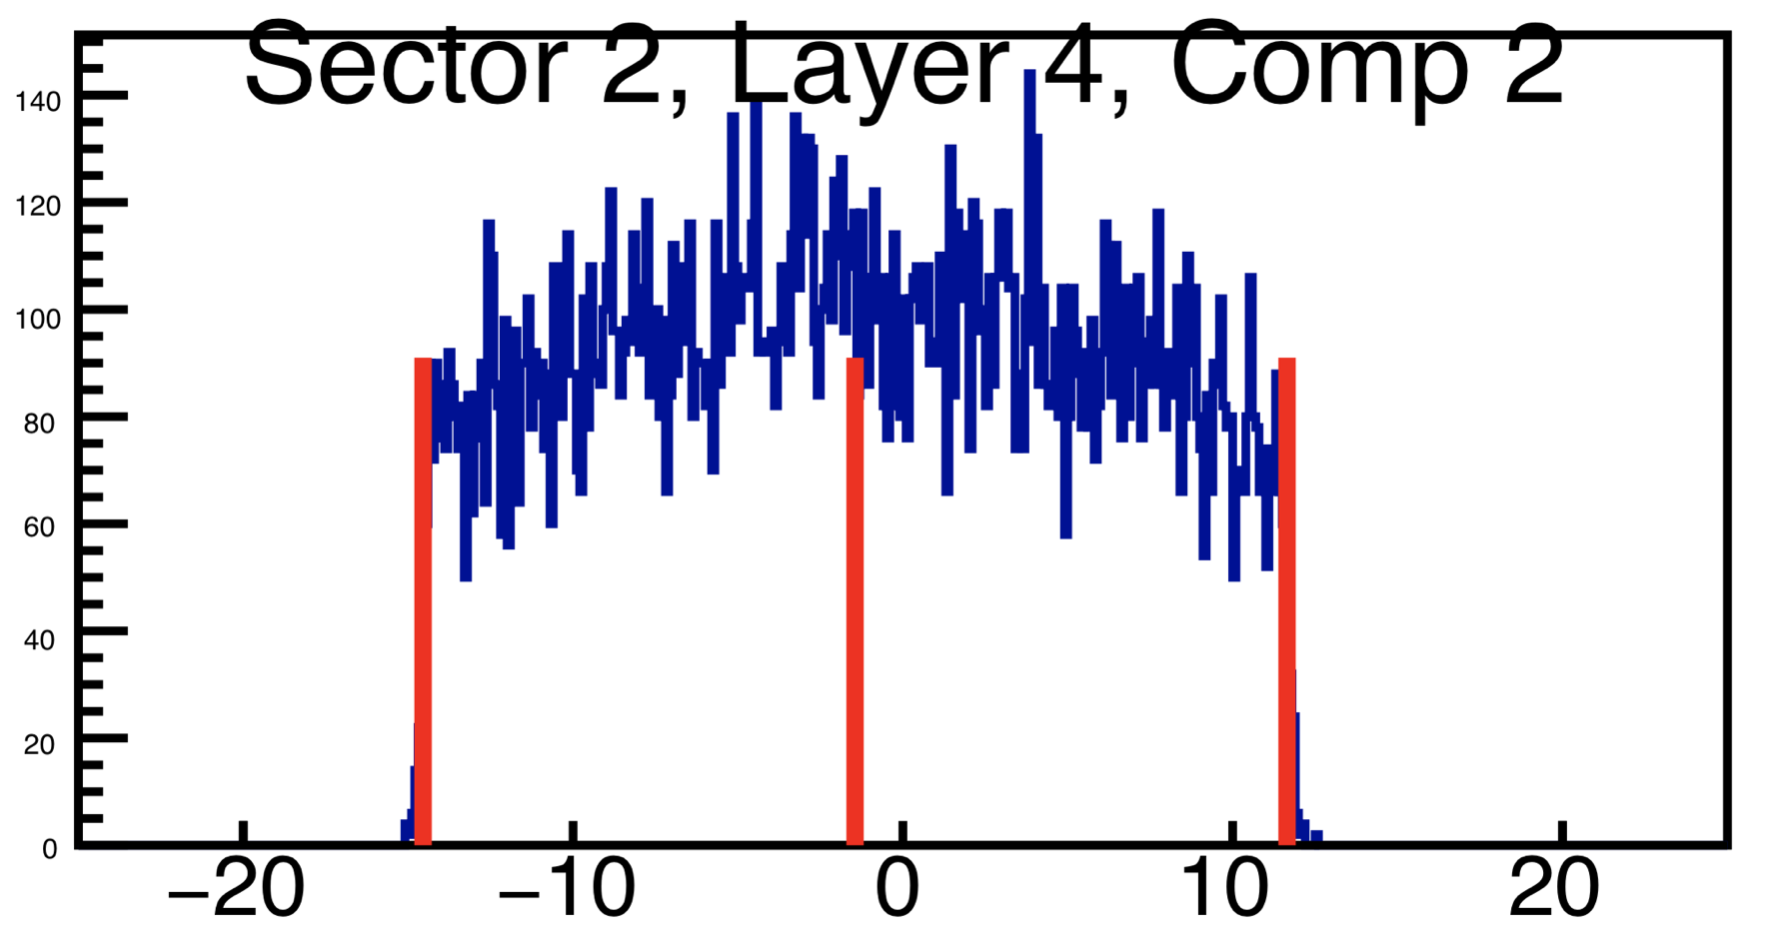
\includegraphics[width=0.48\textwidth]{lr_eff_vel.png}
		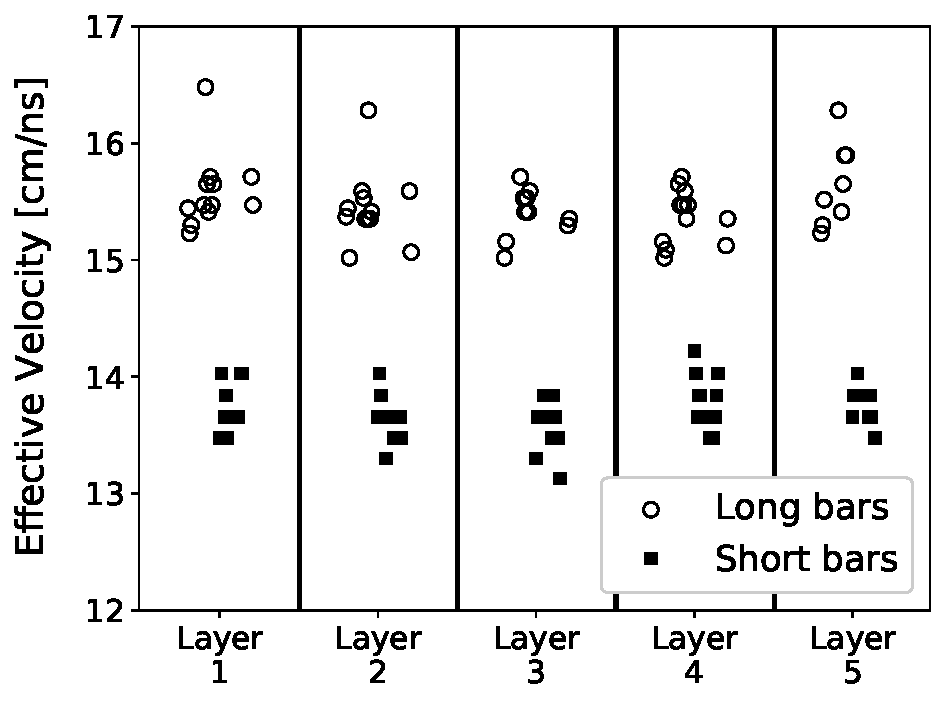
\includegraphics[width=0.48\textwidth]{eff_vel.pdf}
	\caption{}
	\label{fig:eff_vel}
\end{figure}

%%% ----------------- Attenuation length subsection
\subsubsection{Attenuation length}
The attenuation length of the scintillator material can be extracted using cosmic ray data by using the 
amplitude ($A$) and time measured by both PMTs in the bar:
\begin{eqnarray}
	\begin{split}
		A_L(x) &= A_0 e^{-\frac{1}{\mu}\left(L/2-x\right) }				\\
		A_R(x) &= A_0 e^{-\frac{1}{\mu}\left(L/2+x\right) }				\\
		R(x) \equiv \ln{\frac{A_L(x)}{A_R(x)}} &= \frac{2x}{\mu},					
		 \label{eqn:atten}
	\end{split}
\end{eqnarray}
where $x=-\frac{v}{2}(t_L - t_R)$. So by measuring the slope of $R(x)$, one can extract the attenuation length 
of the bar. See Fig.~\ref{fig:atten} for the typical response of a bar to cosmic ray data, and the resulting attenuation 
length. {\color{red}A comparison of the attenuation lengths of all bars can be seen in Fig.~\ref{fig:atten_allbars}}.

\begin{figure}[h!]
	\centering
		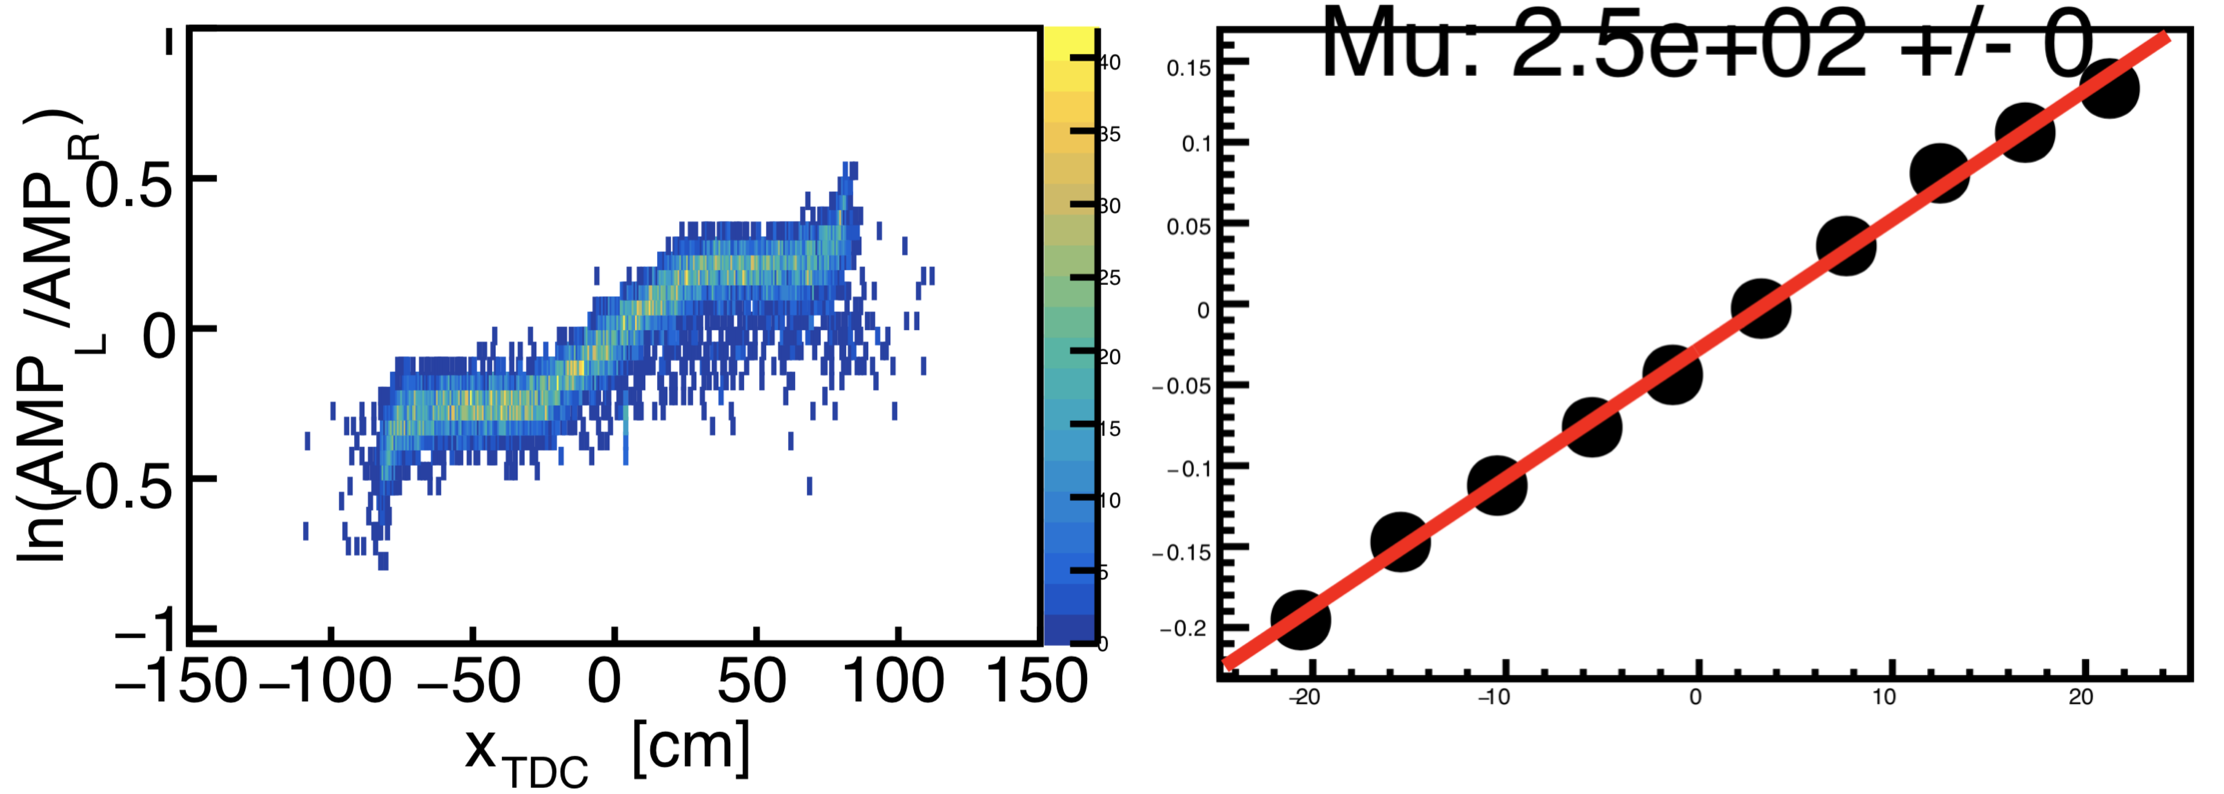
\includegraphics[width=0.96\textwidth]{atten.png}
	\caption{}
	\label{fig:atten}
\end{figure}

%%% ----------------- Bar offsetts subsection
\subsubsection{Bar offsets}
After all bars are individually calibrated, relative time delays between bars can still remain, and require correction to combine 
statistics from all bars. The alignment of all bars can be done quickly using the laser calibration system, as the laser pulse arrival 
time to each bar should be within timing resolution, provided all of the fiber optic cables are of the same length to the BAND bars. 
However, the $51$ \si{\centi\meter} bars have fiber optic cables of $1.5$ \si{\meter} length from the patch panel to the center 
of the bars, and the $160$ and $200$  \si{\centi\meter} bars have fiber optic cables of $2.5$ \si{\meter} length. This residual offset 
between the ``short" bars and ``long" bars can be corrected later by using the photon arrival time to the bars with production data, 
grouping the short bars and long bars separately (see later). Furthermore, obtaining bar alignment with only production data 
requires high-statistics datasets due to the backward-angle placement of the BAND. 

Using data taken with the laser calibration system, bar alignment is done on the average time of a given bar, 
$t_{avg,i} = \frac{1}{2} \left(t_L + t_R\right)_i$. An offset is extracted for each bar relative to a reference bar in it's 
layer, and each reference bar relative to the most downstream layer. For example, the alignment for bar $i$ in layer
$j$ is done as follows:
\begin{eqnarray}
	\begin{split}
		\mathcal{O}^{ij} 	&= \braket{ t_{avg}^i - t_{avg}^{j}  }				\\
		\mathcal{O}^{j} 		&= \braket{ t_{avg}^j - t_{avg}^{ref}  }				\\
		t^{i,j}_{corr} 		&=  t_{avg}^i - \mathcal{O}^{ij}  - \mathcal{O}^{j},
		\label{eqn:atten}
	\end{split}
\end{eqnarray}
where $ t_{avg}^{ref}$ is the average time of the global reference bar chosen on the most downstream layer of the BAND, and
$t_{avg}^j$ is the average time of the reference bar chosen in layer $j$. Then only one global offset is needed to correct the
offset of $t_{avg}^j$ (expect, as mentioned, an additional correction is needed for the long and short bars due to the fiber optic 
cable time difference). Fig~\ref{fig:bar_off} shows a typical relative timing distribution of the bar with respect to a reference bar 
in the same layer, as a function of pulse amplitude. The mean of this distribution is $\mathcal{O}^{ij}$ for this bar, and the 
parameter's independence of pulse amplitude ensures the bar's time-walk is well controlled.

\begin{figure}[h!]
	\centering
		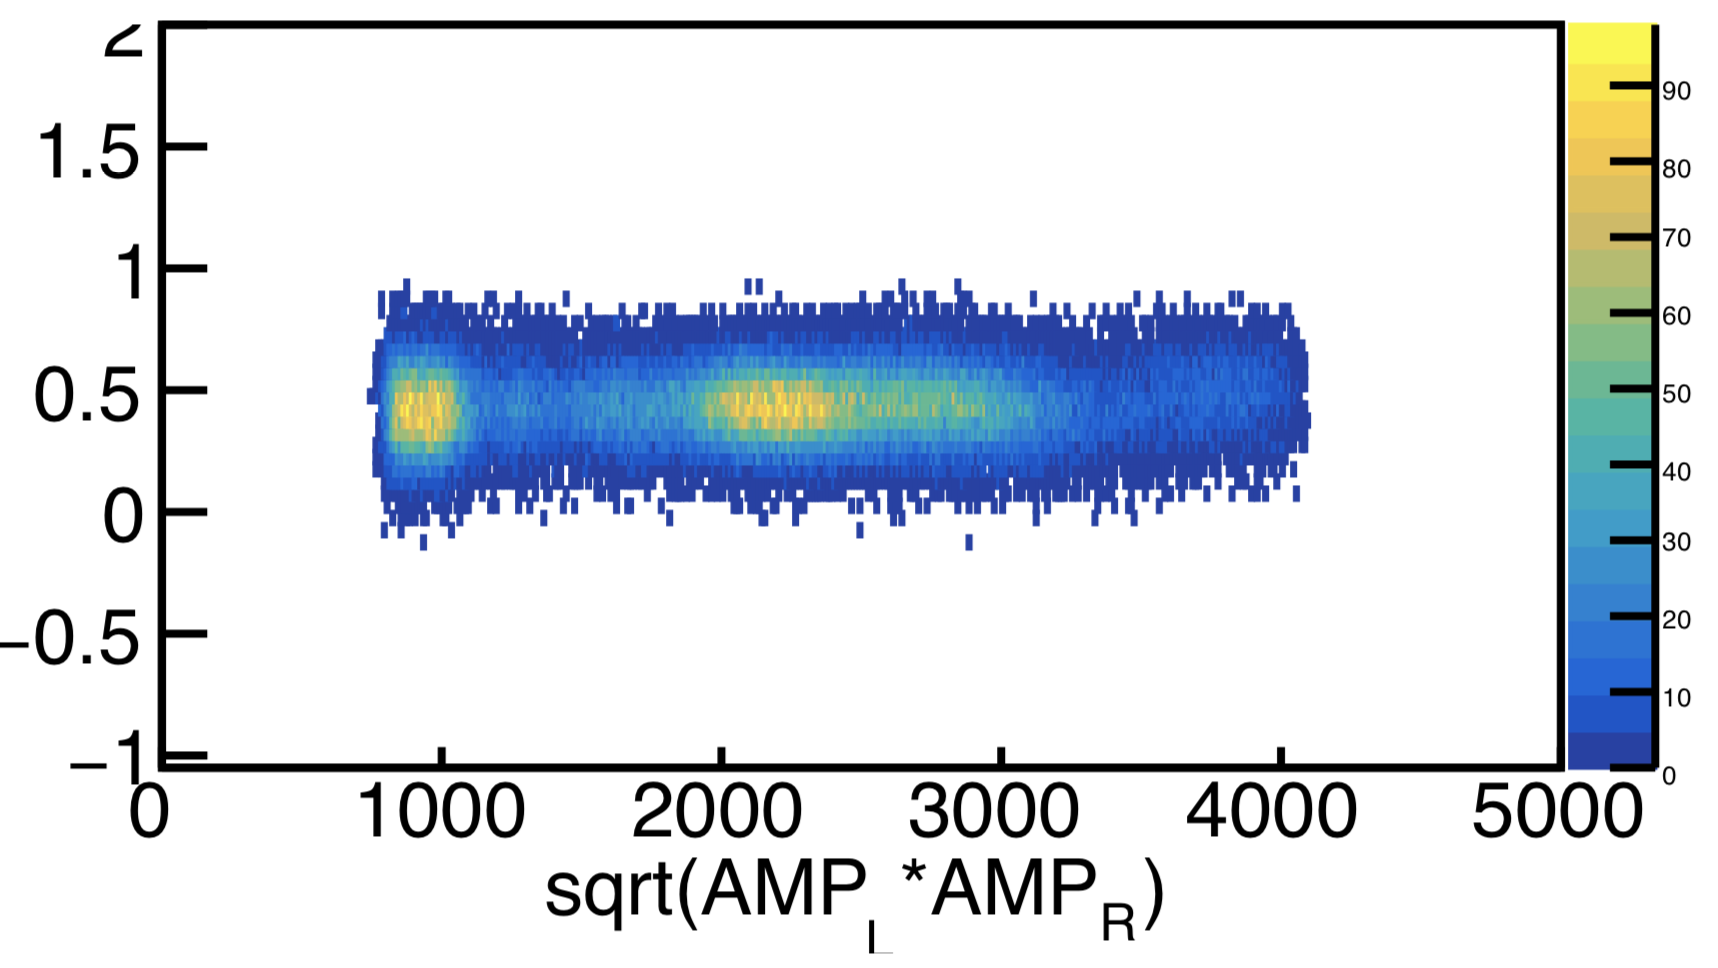
\includegraphics[width=0.8\textwidth]{bar_offset.png}
	\caption{}
	\label{fig:bar_off}
\end{figure}

\subsection{BAND performance} 
%%% ----------------- Global offset subsection
\subsubsection{Global offset}
A final global time offset is required to align the BAND with production data. Due to low rates in the angular coverage of the BAND, 
high-statistics data files must be used. 
Fig.~\ref{fig:final_offset}
\begin{figure}[h!]
	\centering
		\includegraphics[width=0.48\textwidth]{global_single_bar_all_runs.pdf}
		\includegraphics[width=0.48\textwidth]{global_all_bars_single_run.pdf}
		\includegraphics[width=0.48\textwidth]{global_single_bar_result.pdf}
		\includegraphics[width=0.48\textwidth]{tof_resolution.pdf}
	\caption{}
	\label{fig:final_offset}
\end{figure}
%%% ----------------- Neutral veto subsection
\subsubsection{Neutral veto algorithm}

%%% ----------------- Photon-neutron subsection
\subsubsection{Neutron identification}
Fig.~\ref{fig:tof}
\begin{figure}[h!]
	\centering
		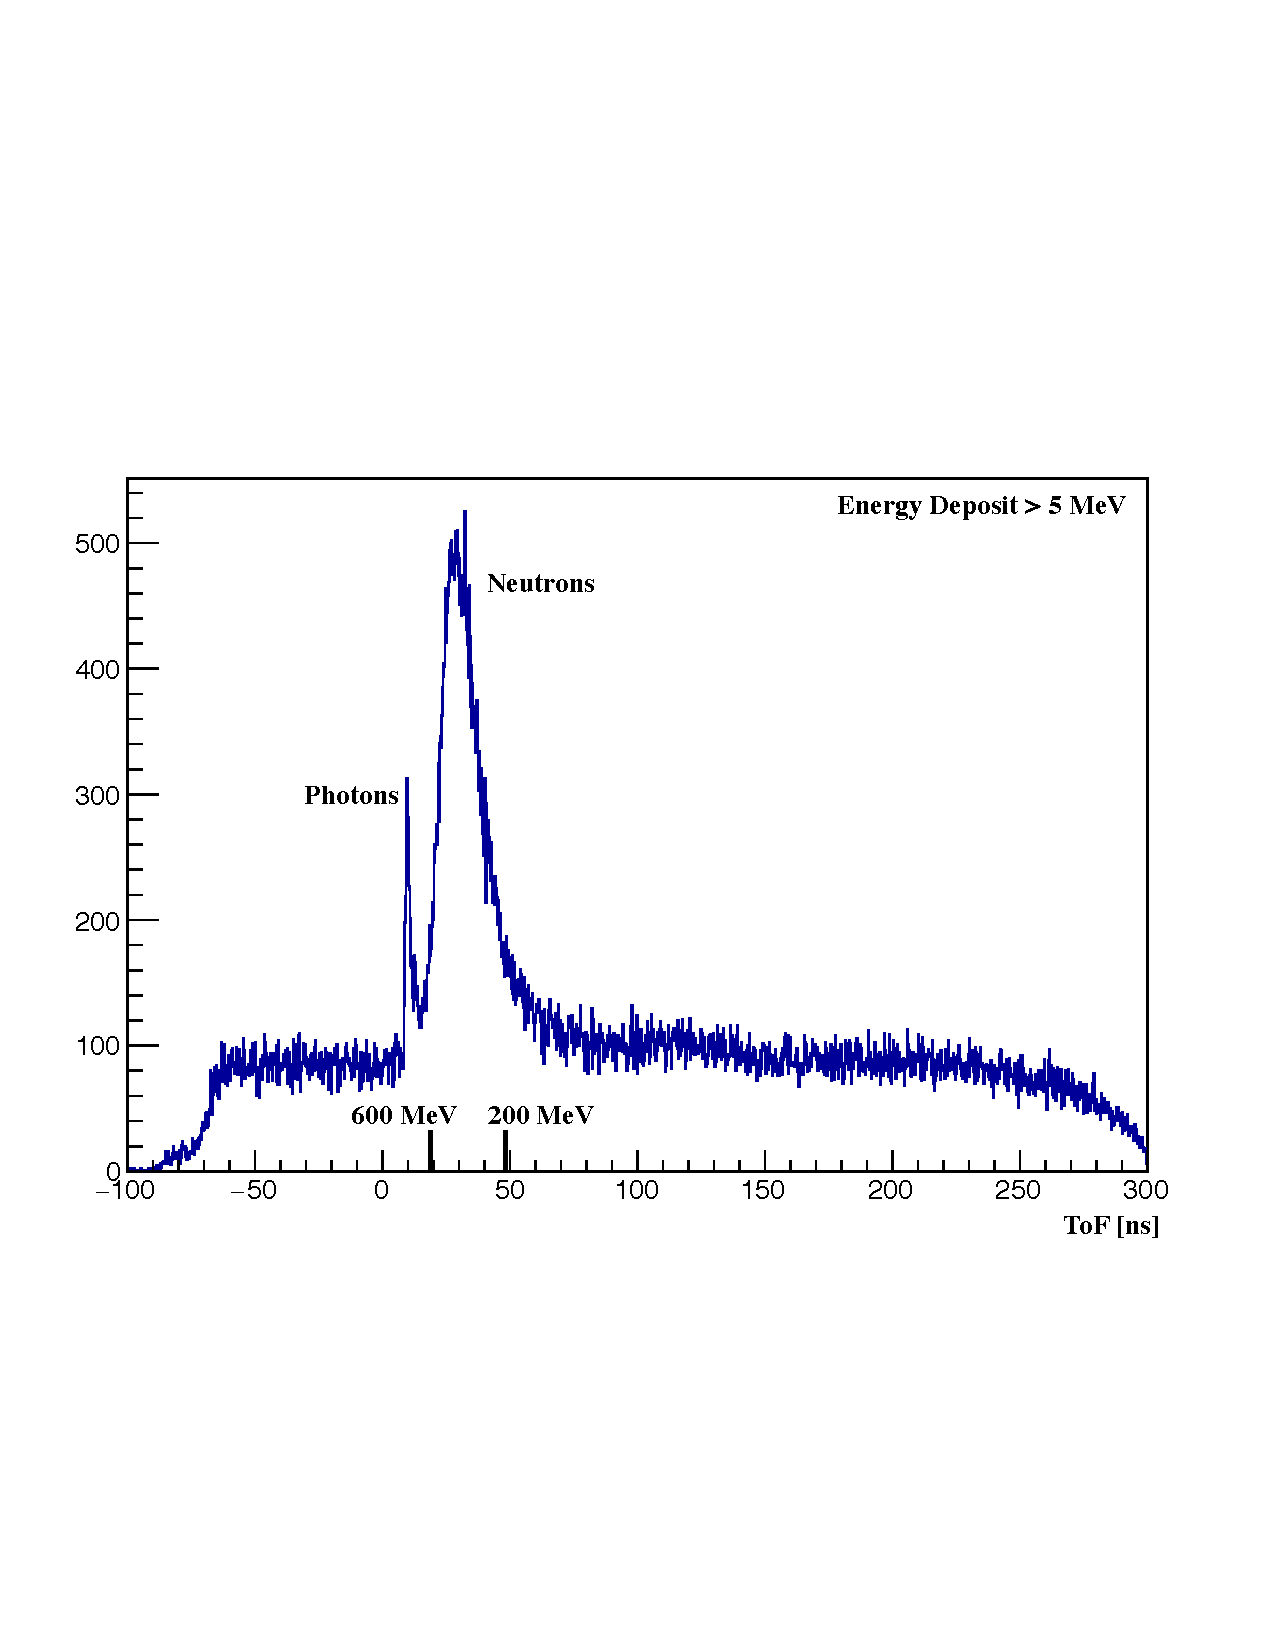
\includegraphics[width=0.96\textwidth]{tof-labels.pdf}
	\caption{}
	\label{fig:tof}
\end{figure}

%%% ----------------- Efficiency, resolution subsection
\subsubsection{Neutron efficiency and resolution}


	



%%%%%%%%%%%%%%%%%%%%%%%%%%%%%%%%%%%%%%%%%%%%%%%%%%%%%%%%%%%%%%%%%%%%%%%%%%%%%%%%%%%%%%%%%%%%%%%%%%%

\section{Summary}

%%%%%%%%%%%%%%%%%%%%%%%%%%%%%%%%%%%%%%%%%%%%%%%%%%%%%%%%%%%%%%%%%%%%%%%%%%%%%%%%%%%%%%%%%%%%%%%%%%%

\section{Acknowledgements}

%%%%%%%%%%%%%%%%%%%%%%%%%%%%%%%%%%%%%%%%%%%%%%%%%%%%%%%%%%%%%%%%%%%%%%%%%%%%%%%%%%%%%%%%%%%%%%%%%%%
\clearpage

\section{Appendix}
\begin{longtable}{  m{3em} | m{3em} | m{5em} | m{3em} | m{3em} | m{3em} | m{8em} }
		\hline
			Sector & Layer & Component & Length (\si{\centi\meter}) & PMTs  & $\sigma$ (\si{\pico\second}) & Nominal distance from target (\si{\centi\meter}) \\
		\hline
		\hline
1	&1	&1	&160	&R7724	&XXX	&XXX\\ 
1	&1	&2	&160	&R7724	&XXX	&XXX\\ 
1	&1	&3	&160	&R7724	&XXX	&XXX\\ 
2	&1	&1	&200	&R7724	&XXX	&XXX\\ 
2	&1	&2	&200	&R7724	&XXX	&XXX\\ 
2	&1	&3	&200	&R7724	&XXX	&XXX\\ 
2	&1	&4	&200	&R7724	&XXX	&XXX\\ 
2	&1	&5	&200	&R7724	&XXX	&XXX\\ 
2	&1	&6	&200	&R7724	&XXX	&XXX\\ 
2	&1	&7	&200	&R7724	&XXX	&XXX\\ 
3	&1	&1	&50	&ET9214	&XXX	&XXX\\ 
3	&1	&2	&50	&ET9214	&XXX	&XXX\\ 
3	&1	&3	&50	&ET9214	&XXX	&XXX\\ 
3	&1	&4	&50	&ET9214	&XXX	&XXX\\ 
3	&1	&5	&50	&ET9214	&XXX	&XXX\\ 
3	&1	&6	&50	&ET9214	&XXX	&XXX\\ 
4	&1	&1	&50	&ET9214	&XXX	&XXX\\ 
4	&1	&2	&50	&ET9214	&XXX	&XXX\\ 
4	&1	&3	&50	&ET9214	&XXX	&XXX\\ 
4	&1	&4	&50	&ET9214	&XXX	&XXX\\ 
4	&1	&5	&50	&ET9214	&XXX	&XXX\\ 
4	&1	&6	&50	&ET9214	&XXX	&XXX\\ 
1	&2	&1	&160	&R7724	&XXX	&XXX\\ 
1	&2	&2	&160	&R7724	&XXX	&XXX\\ 
1	&2	&3	&160	&R7724	&XXX	&XXX\\ 
2	&2	&1	&200	&R7724	&XXX	&XXX\\ 
2	&2	&2	&200	&R7724	&XXX	&XXX\\ 
2	&2	&3	&200	&R7724	&XXX	&XXX\\ 
2	&2	&4	&200	&R7724	&XXX	&XXX\\ 
2	&2	&5	&200	&R7724	&XXX	&XXX\\ 
2	&2	&6	&200	&R7724	&XXX	&XXX\\ 
2	&2	&7	&200	&R7724	&XXX	&XXX\\ 
3	&2	&1	&50	&ET9214	&XXX	&XXX\\ 
3	&2	&2	&50	&ET9214	&XXX	&XXX\\ 
3	&2	&3	&50	&ET9214	&XXX	&XXX\\ 
3	&2	&4	&50	&ET9214	&XXX	&XXX\\ 
3	&2	&5	&50	&ET9214	&XXX	&XXX\\ 
3	&2	&6	&50	&ET9214	&XXX	&XXX\\ 
4	&2	&1	&50	&ET9214	&XXX	&XXX\\ 
4	&2	&2	&50	&ET9214	&XXX	&XXX\\ 
4	&2	&3	&50	&ET9214	&XXX	&XXX\\ 
4	&2	&4	&50	&ET9214	&XXX	&XXX\\ 
4	&2	&5	&50	&ET9214	&XXX	&XXX\\ 
4	&2	&6	&50	&ET9214	&XXX	&XXX\\ 
1	&3	&1	&160	&R7724	&XXX	&XXX\\ 
1	&3	&2	&160	&R7724	&XXX	&XXX\\ 
1	&3	&3	&160	&R7724	&XXX	&XXX\\ 
2	&3	&1	&200	&R7724	&XXX	&XXX\\ 
2	&3	&2	&200	&R7724	&XXX	&XXX\\ 
2	&3	&3	&200	&R7724	&XXX	&XXX\\ 
2	&3	&4	&200	&R7724	&XXX	&XXX\\ 
2	&3	&5	&200	&R7724	&XXX	&XXX\\ 
2	&3	&6	&200	&R7724	&XXX	&XXX\\ 
2	&3	&7	&200	&R7724	&XXX	&XXX\\ 
3	&3	&1	&50	&ET9214	&XXX	&XXX\\ 
3	&3	&2	&50	&ET9214	&XXX	&XXX\\ 
3	&3	&3	&50	&ET9214	&XXX	&XXX\\ 
3	&3	&4	&50	&ET9214	&XXX	&XXX\\ 
3	&3	&5	&50	&ET9214	&XXX	&XXX\\ 
3	&3	&6	&50	&ET9214	&XXX	&XXX\\ 
4	&3	&1	&50	&ET9214	&XXX	&XXX\\ 
4	&3	&2	&50	&ET9214	&XXX	&XXX\\ 
4	&3	&3	&50	&ET9214	&XXX	&XXX\\ 
4	&3	&4	&50	&ET9214	&XXX	&XXX\\ 
4	&3	&5	&50	&ET9214	&XXX	&XXX\\ 
4	&3	&6	&50	&ET9214	&XXX	&XXX\\ 
1	&4	&1	&160	&R7724	&XXX	&XXX\\ 
1	&4	&2	&160	&R7724	&XXX	&XXX\\ 
1	&4	&3	&160	&R7724	&XXX	&XXX\\ 
2	&4	&1	&200	&R7724	&XXX	&XXX\\ 
2	&4	&2	&200	&R7724	&XXX	&XXX\\ 
2	&4	&3	&200	&R7724	&XXX	&XXX\\ 
2	&4	&4	&200	&R7724	&XXX	&XXX\\ 
2	&4	&5	&200	&R7724	&XXX	&XXX\\ 
2	&4	&6	&200	&R7724	&XXX	&XXX\\ 
2	&4	&7	&200	&R7724	&XXX	&XXX\\ 
3	&4	&1	&50	&ET9214	&XXX	&XXX\\ 
3	&4	&2	&50	&ET9214	&XXX	&XXX\\ 
3	&4	&3	&50	&ET9214	&XXX	&XXX\\ 
3	&4	&4	&50	&ET9214	&XXX	&XXX\\ 
3	&4	&5	&50	&ET9214	&XXX	&XXX\\ 
3	&4	&6	&50	&ET9214	&XXX	&XXX\\ 
4	&4	&1	&50	&ET9214	&XXX	&XXX\\ 
4	&4	&2	&50	&ET9214	&XXX	&XXX\\ 
4	&4	&3	&50	&ET9214	&XXX	&XXX\\ 
4	&4	&4	&50	&ET9214	&XXX	&XXX\\ 
4	&4	&5	&50	&ET9214	&XXX	&XXX\\ 
4	&4	&6	&50	&ET9214	&XXX	&XXX\\ 
		\hline
	\end{longtable}




\section*{References}

% Create the reference section using BibTeX:
\bibliography{band_nim_bib}


\end{document}
